\makeatletter\let\ifGm@compatii\relax\makeatother
% Problemas con el paquete geometry se solucionan con la anterior
% sentencia. 18/5/2015
\documentclass[8pt]{beamer}

\usetheme{Warsaw}

\usecolortheme{beaver}

%\usepackage[utf8]{inputenc}
\usepackage[latin1]{inputenc}
\usepackage[greek, spanish]{babel}

\usepackage{acronym}	% Acronimos

\usepackage{graphicx}
\usepackage{epstopdf}
\usepackage{multicol}
\usepackage{multirow}
\usepackage{hyperref}
\usepackage{url}
\usepackage{multicol}

\usepackage{appendix}
\usepackage{pdflscape}	%rotacion 90� paginas y las muestra rotadas
\usepackage[square]{natbib}
\usepackage{rotating}

%-----------------paquetes graficos
\usepackage[tikz]{bclogo}


\epstopdfDeclareGraphicsRule{.gif}{png}{.png}{%
  convert gif:#1 png:\OutputFile
}
\AppendGraphicsExtensions{.gif}


\newcommand{\gt}{>}

\newcommand{\griego}[1]{
	\begin{otherlanguage}{greek}
	#1
	\end{otherlanguage}
      }


%-----------------Titulo y autores

\title{Cap\'itulo 1 \\
	Paneles de Instrumentos}
\subtitle{C\'atedra de Instrumentos y Avi\'onica}
\author{ Ing. Jorge Garcia}
\institute{
	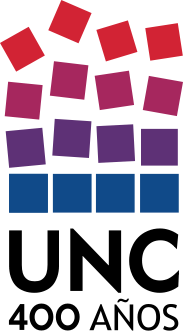
\includegraphics[height=1.5cm]{imagenes/logos/400-anios} \hspace{3mm}	
	
\includegraphics[height=1cm]{imagenes/logos/logoUNC} \hspace{1mm}	
	
\includegraphics[height=1cm]{imagenes/logos/fcefyn} \hspace{1mm}	
	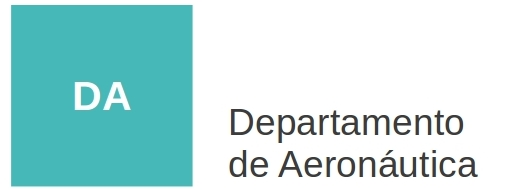
\includegraphics[height=1cm]{imagenes/logos/dpto-aero-logo}
	\\
%	Departamento de Aeron\'autica \\
%	Facultad de Ciencias Exactas, F\'isicas y Naturales \\
%	Universidad Nacional de C\'ordoba
	}
\date{A\~no 2019}


%----------------------------------CONTENIDO------------------

% Capi�tulo 1. Paneles de Instrumentos
% 1.1. Introduccion al estudio del instrumental.
% 1.2. Clasificacion de los Instrumentos.
% 1.3. Distribucion Normalizada del Instrumental en el Tablero
% 1.4. Presentacion en Pantalla Electronica.

\begin{document}

%----------- titlepage -----------%
\begin{frame}[plain]
  \titlepage
\end{frame}

\section{Paneles de instrumentos}
\label{sec:paneles.instrumentos}

\begin{frame}{Paneles de instrumentos}

\tableofcontents[pausesections]
  
\end{frame}


\subsection{Introducci\'on al estudio del instrumental}
\label{sec:cap.1.1.introduccion.estudio.instrumental}

	% Version 2019

\subsubsection{Instrumentos de vuelo}
\label{sec:instrumentos.de.vuelo}


\begin{frame}{Instrumentos de vuelo}

  \begin{block}{Instrumento}
    Del lat. instrumentum.\\
    m. Objeto fabricado, relativamente sencillo, con el que se puede realizar una actividad.\\
   {\tiny Fuente: Diccionario R.A.E.}
  \end{block}

  \begin{columns}{2}

    \begin{column}{0.5\textwidth}

{\small


  \begin{block}{Instrumentos de vuelo}
	Conjunto de mecanismos y dispositivos que forman parte de una aeronave y 
	que posibilitan que un vuelo se lleve a cabo en condiciones seguras.\\
	{\tiny Fuente: \url{https://definicion.de/instrumento/}}
  \end{block}


  \begin{block}{    Necesidades a cumplir:}
    \begin{itemize}
    \item Permitir volar en condiciones de clim\'aticas desfavorables, 
	con escasa visibilidad y durante la noche
    \item Asegurar una operaci\'on segura y confiable
    \item Dar avisos tempranos sobre cualquier falla en los sistemas
      de la aeronave o partes de la misma, de forma que los pilotos
      puedan tomar una acci\'on inmediata
    \end{itemize}
  \end{block}
}
\end{column}
    \begin{column}{0.5\textwidth} \centering
 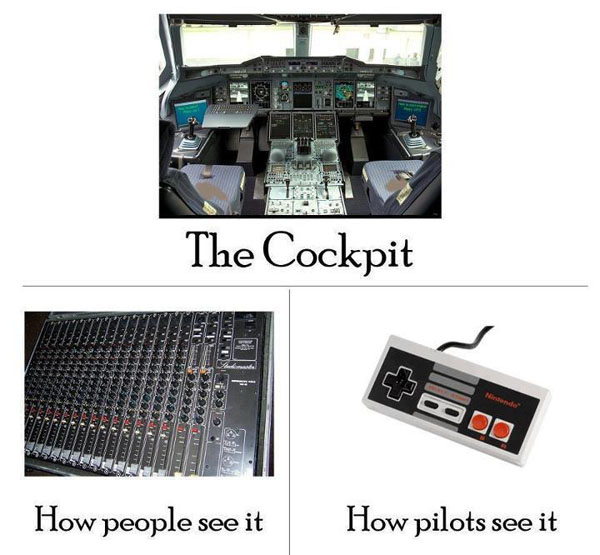
\includegraphics[width=\linewidth]{imagenes/1.1.introduccion/TheCockpit.jpg} \\
{\tiny Fuente: \url{https://aviationhumor.net/flight-deck-cockpit-jokes-and-memes/}}
    \end{column}
  \end{columns}

\end{frame}

\begin{frame}{Evoluci\'on en el tiempo de las cabinas de vuelo} \centering
   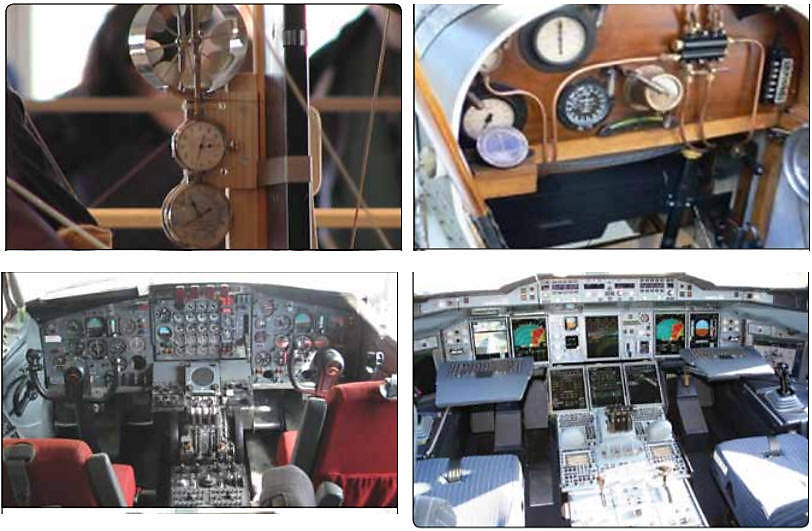
\includegraphics[height=0.6\linewidth, width=0.9\linewidth]{imagenes/1.1.introduccion/evolucion_cabina.jpg} \\
{\footnotesize Arriba izquierda: Wright Flyer, Arriba derecha: avi\'on primera guerra mundial, \\
Abajo izquierda: Boeing 707 entre los '60 y '70, Abajo derecha: Airbus A380.}\\
{\tiny Fuente: \url{https://www.waybuilder.net/free-ed/SkilledTrades/Aviation/AvAirframes/10AiInstrumt/10AiInstrumtFra.asp}}
\end{frame}

\begin{frame}
  
  \begin{alertblock}{}
    La habilidad de capturar y transmitir toda la informaci\'on que un piloto requiere, de forma segura y f\'acil de entender, ha sido un desaf\'io a trav\'es de la historia de la aviaci\'on.\\
{\tiny Referencia:  \cite{FAA_hdk_aMThA_v2}}
  \end{alertblock}

        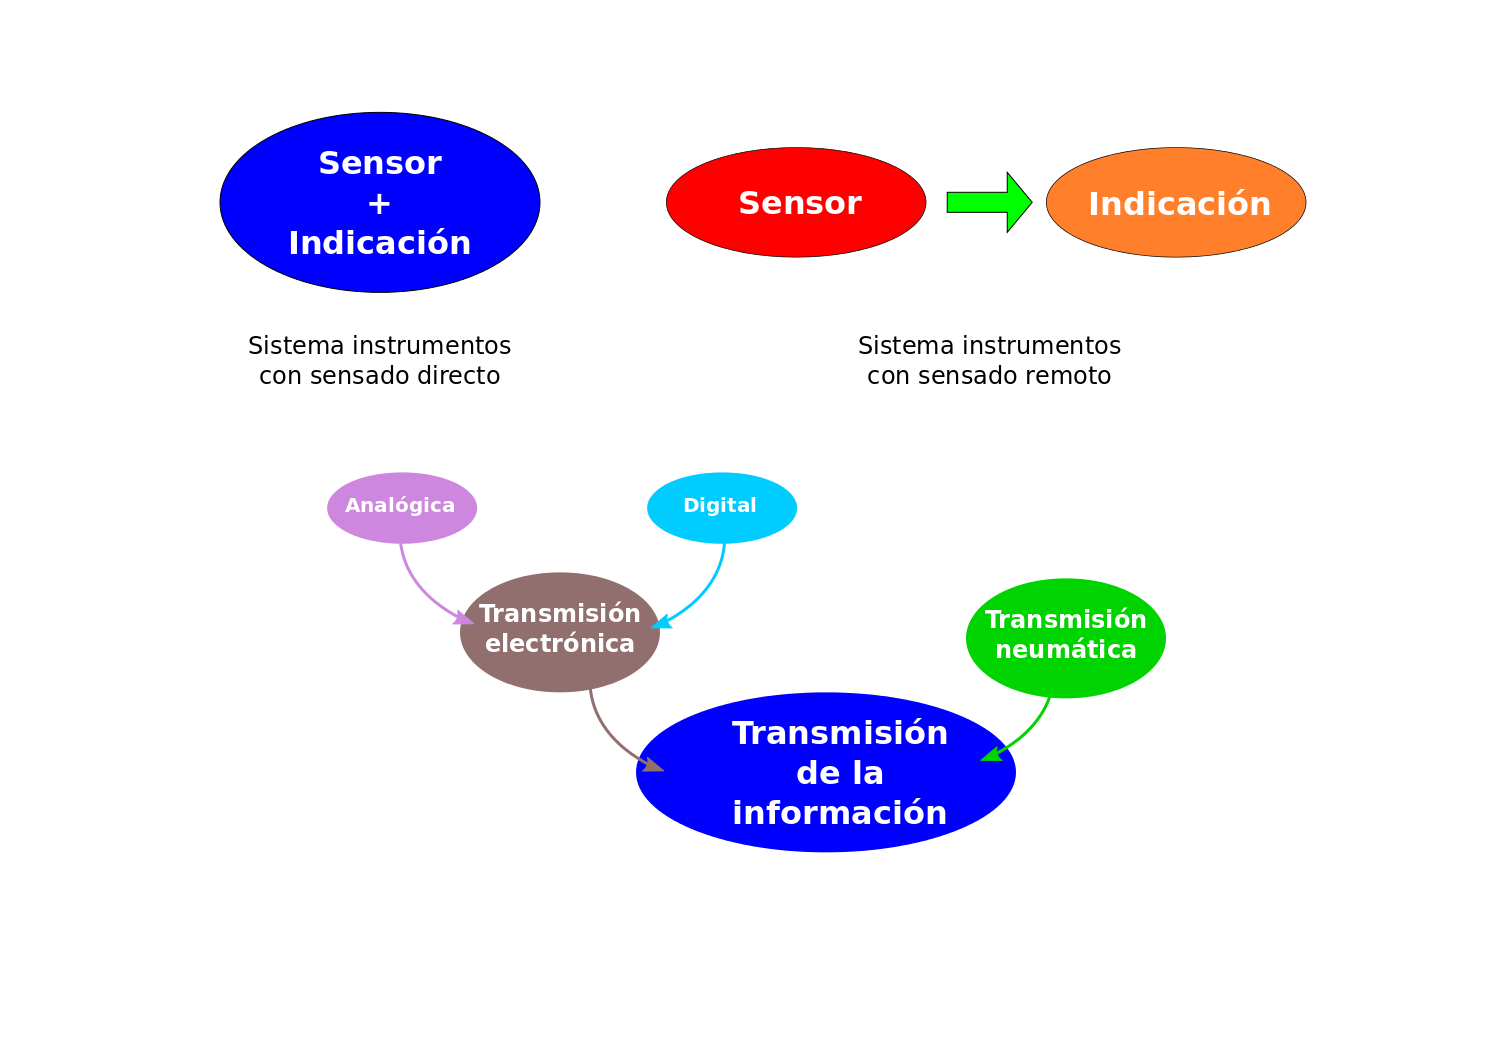
\includegraphics[width=0.9\textwidth]{tikz/01_sistema_instrumentos.png}

        {\tiny Adaptado de: \cite{FAA_hdk_aMThA_v2}}

\end{frame}

\subsubsection{Ergonom\'ia}
\label{sec:ergonomia}

%	01.01.01.Ergonomia
%	version 2019

\begin{frame}

      \begin{block}{Ergonom\'ia}
        \emph{Del gr. 
	\griego{\'ergon}
''ergon'' (trabajo) y 
``nom\'ia'' ( \griego{n\'omos} ``nomos'' (regla, ley), 
	m\'as el sufijo ``ia'' (cualidad))}\\
1. f. Estudio de la adaptaci\'on de las m\'aquinas, muebles y utensilios a la persona que los emplea habitualmente, para lograr una mayor comodidad y eficacia.\\
2. f. Cualidad de ergon\'omico (adaptado a las condiciones del usuario). \emph{El puesto de conducci\'on tiene buena ergonom\'ia.}

{\tiny Fuente: Real Academia Espa\~nola }

\vspace{3mm}

\emph{La Ergonom\'ia (o Factores Humanos) es la disciplina cient\'ifica relacionada con la comprensi\'on de las interacciones entre los seres humanos y los elementos de un sistema, y la profesi\'on que aplica teor\'ia, principios, datos y m\'etodos de dise\~no para optimizar el bienestar humano y todo el desempe\~no del sistema.
}

{\tiny Fuente: Asociaci\'on Internacional de Ergonom\'iía (IEA) \,
\url{https://www.iea.cc/whats/}}
      \end{block}

\end{frame}

\begin{frame}{}
  \begin{block}{Ergonom\'ia Cognitiva}
    ``Se ocupa de los procesos mentales, tales como la percepci\'on, la memoria, el razonamiento y la respuesta motora, que afectan a las interacciones entre los seres humanos y otros elementos de un sistema. %Los temas relevantes incluyen carga de trabajo mental, la toma de decisiones, el rendimiento experto, la interacci\'on persona-computadora, la fiabilidad humana, el estr\'es laboral y la forma como estos pueden estar relacionados con el dise\~no de los sistemas humanos. La ergonom\'ia cognitiva estudia los procesos de cognición en el trabajo y ajustes operativos, a fin de optimizar el bienestar humano y el rendimiento del sistema
"

{\tiny Fuente: Asociaci\'on Internacional de Ergonom\'iía (IEA) \,
\url{https://www.iea.cc/whats/}}

  \end{block}

\vspace{3mm}

El campo de la ergonom\'ia cognitiva surgi\'o predominantemente en los a\~nos 70 con la llegada de la computadora personal y los nuevos desarrollos en los campos de la psicolog\'ia cognitiva y la inteligencia artificial. Se contrasta con la tradici\'on de la ergonom\'ia f\'isica porque ``\emph{la ergonom\'ia cognitiva es... la aplicaci\'on de la psicolog\'ia al trabajo... para lograr la optimizaci\'on entre la gente y su trabajo.}''

{\tiny Fuente: \url{https://es.wikipedia.org/wiki/Ergonom\%C3\%ADa_cognitiva}}

\vspace{3mm}

Mayores detalles pueden consultarse en \cite{van_der_Veer} \\
{\tiny \url{https://pdfs.semanticscholar.org/ea75/ca4d902bc5089c8542751e7ed03c97c13197.pdf}
}


\end{frame}

   
\begin{frame}{Modelo de procesamiento de informaci\'on humano}

  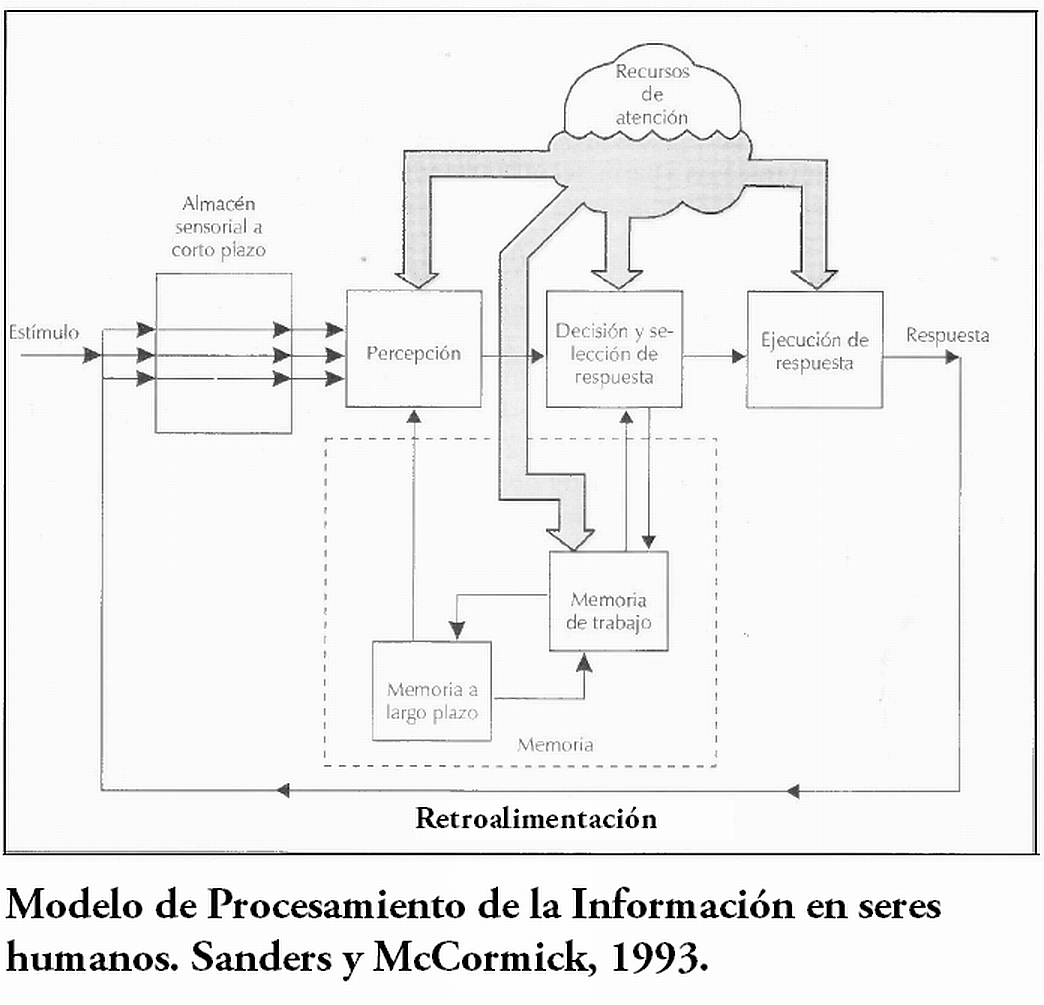
\includegraphics[width=0.6\linewidth]{imagenes/1.1.introduccion/modelo_procesamiento_informacion.png}

{\tiny Fuente: Romosquera, \url{https://commons.wikimedia.org/wiki/File:Procesamiento_de_la_Informaci\%C3\%B3n.png}
\\ \cite{mark1993human} }

\end{frame}

\begin{frame}{Ergonom\'ia F\'isica}
  
La ergonom\'ia f\'isica se ocupa de las caracter\'isticas anat\'omicas, antropom\'etricas, fisiol\'ogicas y biomec\'anicas del usuario, en tanto que se relacionan con la actividad f\'isica.

Sus temas m\'as relevantes incluyen posturas de trabajo, sobreesfuerzo, manejo manual de materiales, movimientos repetitivos, lesiones m\'usculo-tendinosas (LMT) de origen laboral, dise\~no de puestos de trabajo, seguridad y salud ocupacional. 

{\tiny Fuente: Wikipedia}


\begin{center}
  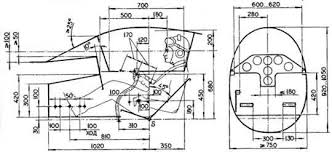
\includegraphics[width=0.7\textwidth]{imagenes/1.1.introduccion/ergonomia_fisica.jpeg}
\end{center}
{\tiny Fuente: \url{https://www.ijsr.net/archive/v6i2/ART2017582.pdf}}


\end{frame}

\begin{frame}{Ergonom\'ia Visual}
  
La ergonom\'ia visual, como dominio dentro de la rama de ergonom\'ia, se centra en recomendaciones b\'asicas que deben cumplir aquellas personas que, en el desempe\~no de su actividad, emplean largas horas trabajando con pantallas y monitores. Estas recomendaciones incluyen aspectos como la separaci\'on entre el usuario y la pantalla, la necesidad de separar la vista del monitor repetidamente y centrarla en un punto lejano, o los beneficios de un parpadeo repetido que hidrate las capas corneales del ojo. 

{\tiny Fuente: Wikipedia}

\begin{center}
  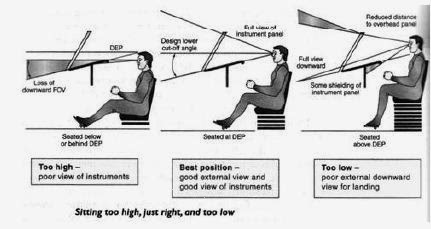
\includegraphics[width=0.7\textwidth]{imagenes/1.1.introduccion/ergonomia_visual.jpg}
\end{center}
{\tiny Fuente: \url{http://avionics-system-design.blogspot.com/2013/12/ergonomics-of-aircraft-cockpit.html}}


\end{frame}



% \begin{frame}

%   \begin{columns}
%     \begin{column}{0.45\textwidth}
%       \begin{block}{Sistema de ciclo cerrado persona-m\'aquina}
%         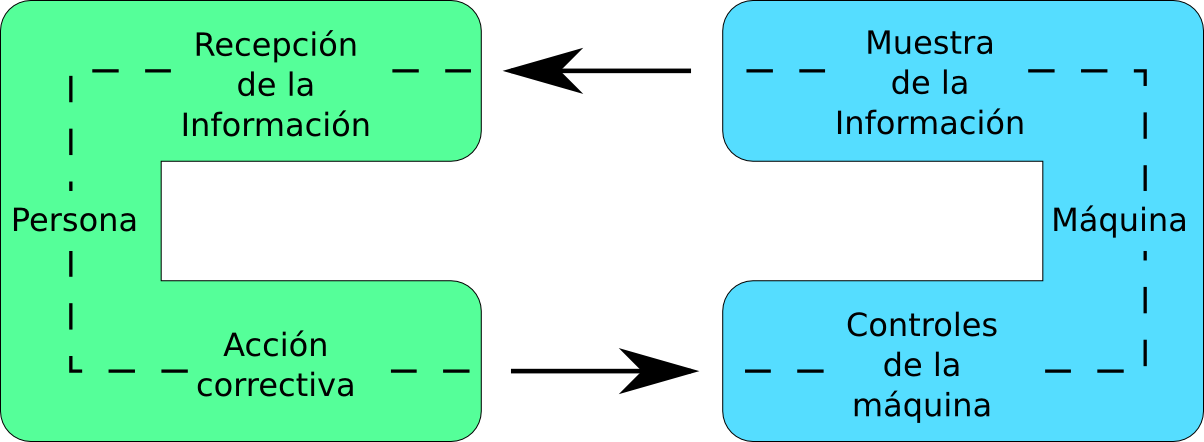
\includegraphics[width=\linewidth]{tikz/01-03-loop-persona-maquina.png}

%         {\tiny Adaptado de \cite{bhandari2010design}}
%       \end{block}
%     \end{column}

%     \begin{column}{0.05\textwidth}
%     \end{column}

%     \begin{column}{0.45\textwidth}

%     \end{column}
      
%   \end{columns}

% \end{frame}



\subsubsection{Formas de presentaci\'on de la informaci\'on}
\label{sec:formas.presentacion.informacion}

%	01.01.01. Formas de presentaci\'on informaci\'on
%	version 2018



\begin{frame}{Formas de presentaci\'on de la informaci\'on}

  \begin{itemize}
  \item {\bf Presentaciones cuantitativas}
    \begin{itemize}
      \item Escala circular
      % \begin{itemize}
      %    \item Escala lineal
      %    \item Escala no lineal (cuadr\'atica, logar\'itmica}
      % \end{itemize}
       \item Escala longitudinal
    \end{itemize}
  \item {\bf Presentaciones cualitativas}
  \item {\bf Presentaciones directoras}
  \end{itemize}

\end{frame}

\begin{frame}{Presentaciones cuantitativas
	}

  \begin{tabular}{ccc}
    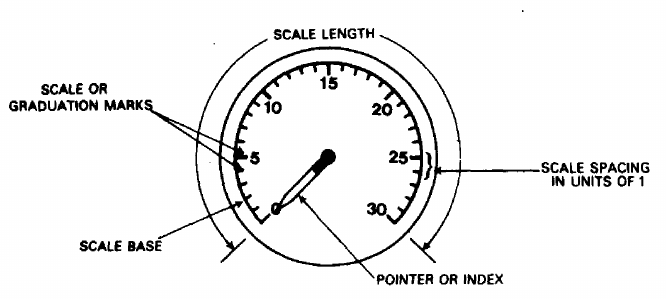
\includegraphics[width=0.45\textwidth]{imagenes/1.2.clasificacion.instrumentos/escala_circular_cuantitativa.png} & \hspace{3mm}
&     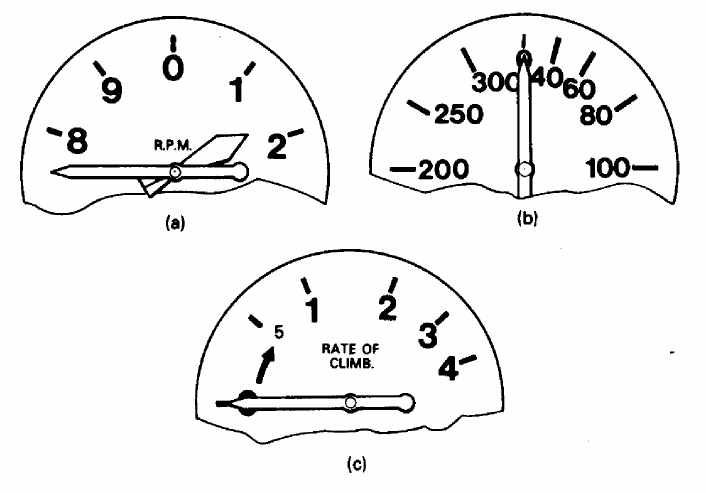
\includegraphics[width=0.45\textwidth]{imagenes/1.2.clasificacion.instrumentos/escala_circular_lineal_no_lineal.png}
\\
	Escala circular cuantitativa & 
& \parbox{0.45\textwidth}{a) Lineal, b) ley cuadr\'atica, \\c) ley logaritmica}
\\
  \end{tabular}

{\tiny Referencia: \cite{pallett1992aircraft}}

\end{frame}

\begin{frame}{Presentaciones cuantitativas
	}

  \begin{tabular}{ccc}
    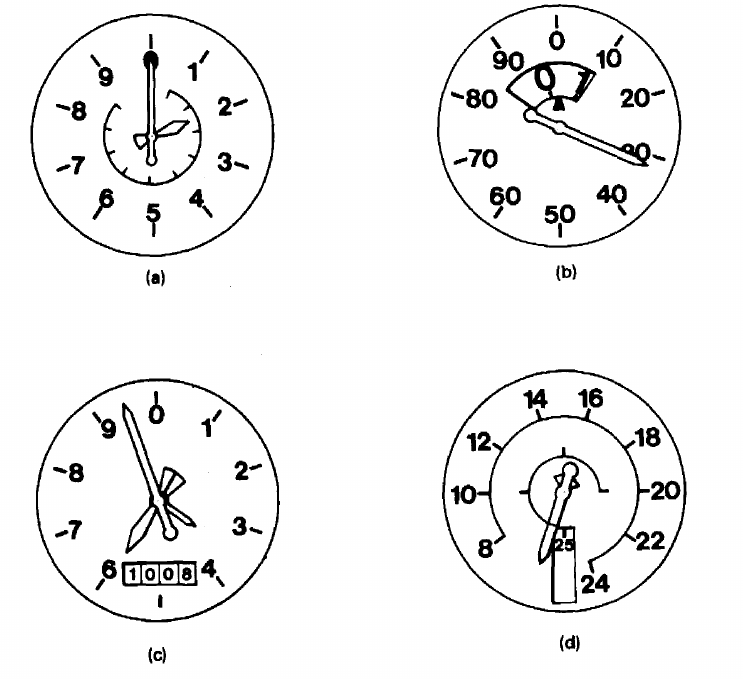
\includegraphics[width=0.45\textwidth]{imagenes/1.2.clasificacion.instrumentos/escala_gran_alcance.png} & \hspace{3mm}
&     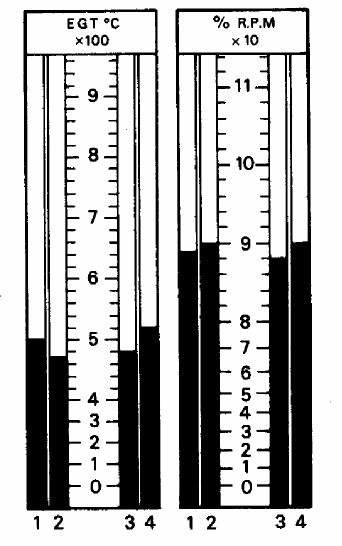
\includegraphics[width=0.35\textwidth]{imagenes/1.2.clasificacion.instrumentos/longitudinal.png}
\\
\parbox{0.45\textwidth}{\small a)Escalas conc\'entricas, (b) escalas fijas y giratorias, (c) escala com\'un tres agujas, (d) aguja dividida}
&
& {\small Escala longitudinal}
\\
  \end{tabular}
{\tiny Referencia: \cite{pallett1992aircraft}}
\end{frame}

\begin{frame}{Clasificaci\'on de los Instrumentos}

  \begin{tabular}{ccc}
    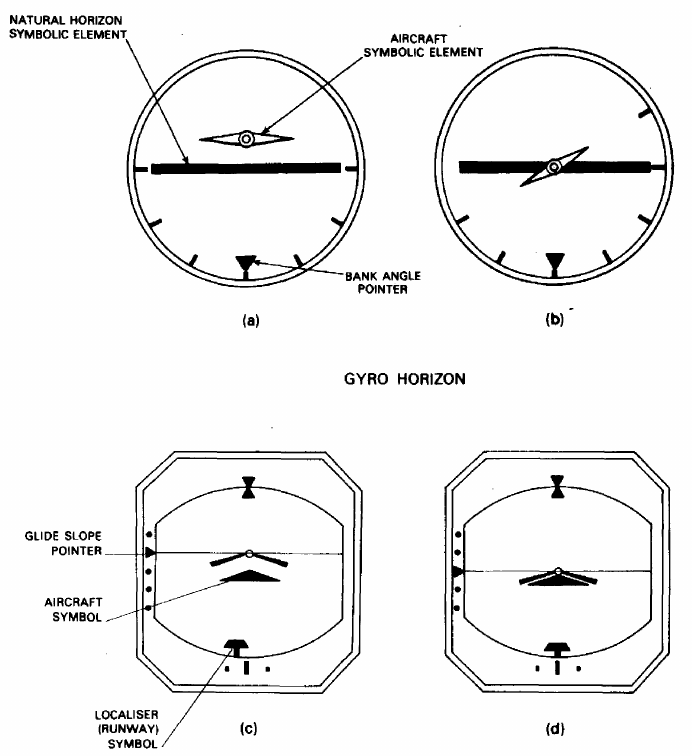
\includegraphics[width=0.45\textwidth]{imagenes/1.2.clasificacion.instrumentos/director.png} & \hspace{3mm}
&     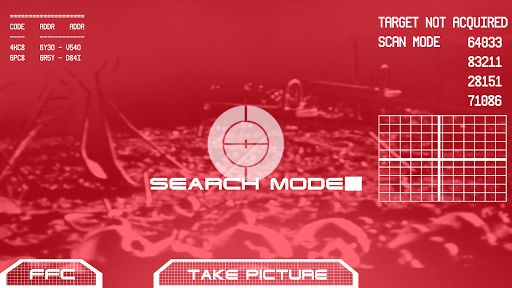
\includegraphics[width=0.5\textwidth]{imagenes/1.2.clasificacion.instrumentos/terminator_hud.png}
\\
\parbox{0.45\textwidth}{Director de vuelo}
&
& Terminator Hud
\\
  \end{tabular}

\end{frame}

\begin{frame}{Clasificaci\'on de los Instrumentos}

{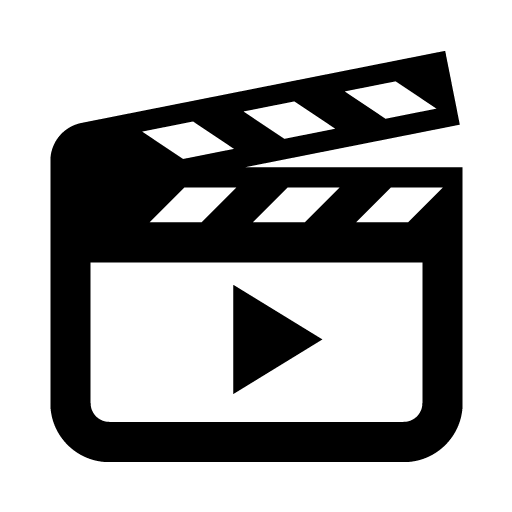
\includegraphics[width=0.1\textwidth]{imagenes/Video.png}}\,
The Evolution of the Head-Up Display \url{https://www.youtube.com/watch?v=ypIbmfm7n8A}
\vspace{3mm}

  \begin{tabular}{ccc}
    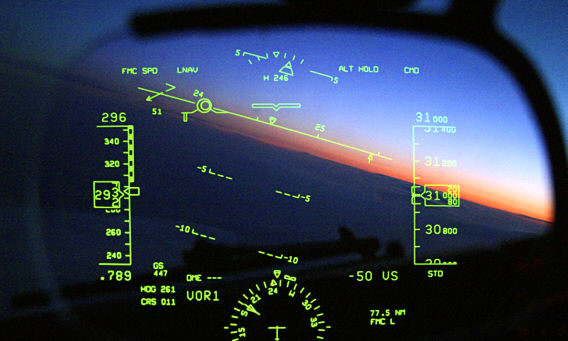
\includegraphics[width=0.45\textwidth]{imagenes/1.2.clasificacion.instrumentos/hud.jpg} & \hspace{3mm}
&     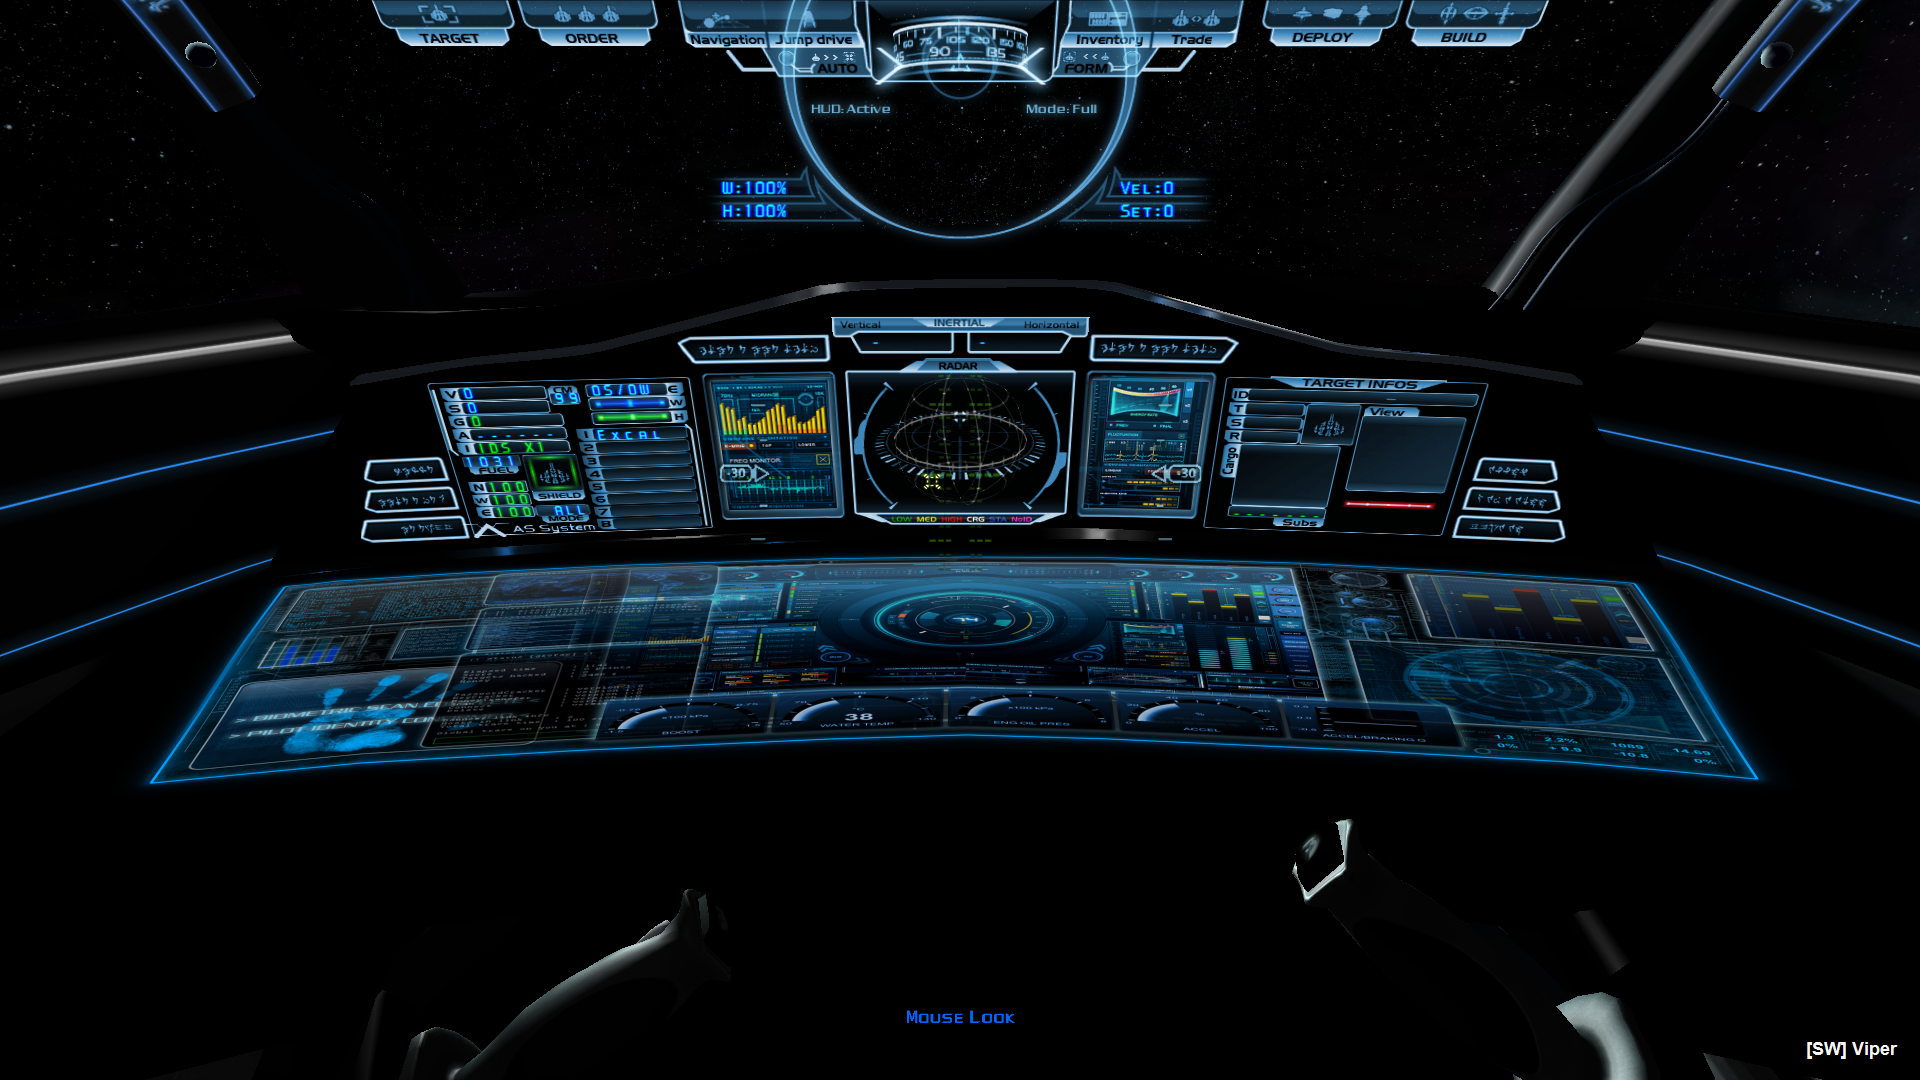
\includegraphics[width=0.5\textwidth]{imagenes/1.2.clasificacion.instrumentos/viper_11.png}
\\
\parbox{0.45\textwidth}{Head Up Display}
&
& Hud futuro
\\
  \end{tabular}

\end{frame}

\begin{frame}{Clasificaci\'on de los Instrumentos}



\vspace{3mm}

{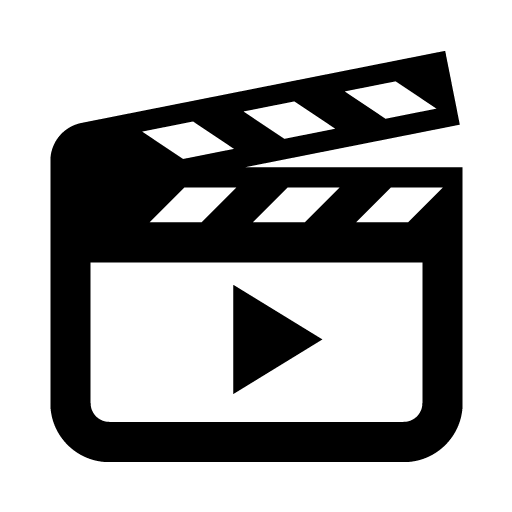
\includegraphics[width=0.1\textwidth]{imagenes/Video.png}}\,
Enhanced Flight Vision System \url{https://www.youtube.com/watch?v=DR9lyAM2YNE}

\vspace{3mm}

  \begin{tabular}{ccc}
    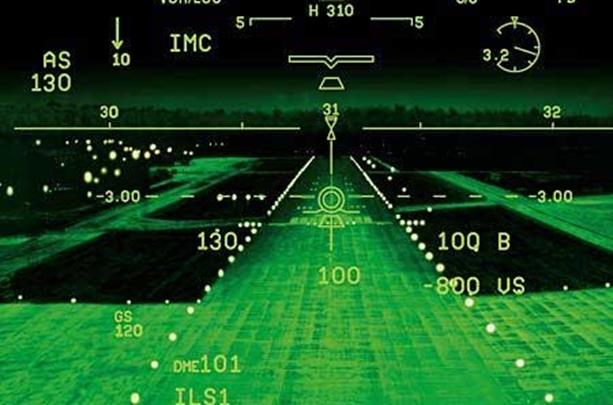
\includegraphics[width=0.45\textwidth]{imagenes/1.2.clasificacion.instrumentos/EFVS_Photo.jpg} & \hspace{3mm}
    &     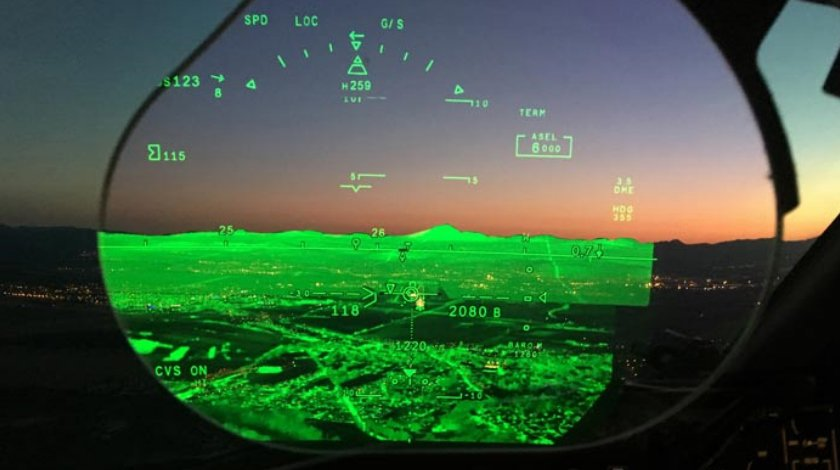
\includegraphics[width=0.45\textwidth]{imagenes/1.2.clasificacion.instrumentos/efvs.jpg} \\
  \end{tabular}
  

\end{frame}


\subsection{Clasificaci\'on de los Instrumentos}
\label{sec:cap.1.2.clasificacion.instrumentos}

%	01.02.Clasificacion instrumentos
%	Version 2018


\begin{frame}{Clasificaci\'on de los Instrumentos}

  \begin{itemize}
  \item {\bf Instrumentos del sistema pitot-est\'atica}
  \item {\bf Instrumentos girosc\'opicos}
  \item {\bf Instrumentos duplicados}
  \item {\bf Instrumentos de navegaci\'on}
  \item {\bf Instrumentos del grupo motopropulsor}
  \end{itemize}

\end{frame}





\begin{frame}{Clasificaci\'on de los Instrumentos}

{\Large \bf Avi\'onica = Aviaci\'on + Electr\'onica}

\end{frame}


\subsection{Distribuci\'on Normalizada del Instrumental en el Tablero}
\label{sec:distribucion.normalizada.instrumental.en.el.tablero}


%	1.3. Distribucion Normalizada del Instrumental en el Tablero
%	version 2018






\begin{frame}{Distribuci\'on Normalizada del Instrumental en el
 Tablero}
  

REGULACIONES ARGENTINAS DE AVIACI\'ON CIVIL (RAAC)\\
PARTE 91 - REGLAS DE VUELO Y OPERACI\'ON GENERAL\\
SUBPARTE C - REQUERIMIENTOS DE EQUIPAMIENTOS, INSTRUMENTOS Y DE
CERTIFICADOS\\

\vspace{3mm}

\colorbox{yellow!30}{\parbox{0.9\textwidth}{{\bf 91.205} \qquad
Requerimientos de instrumentos y equipamiento para aeronaves civiles motorizadas con
Certificado de Aeronavegabilidad Est\'andar de la Rep\'ublica Argentina}
}

\href{run:biblio/parte-91-19feb2016-res-77-16.pdf}{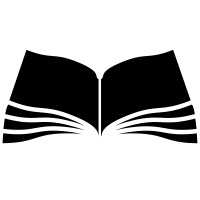
\includegraphics[width=0.1\textwidth]{imagenes/libro.png}}
\hspace{3mm}
\href{http://www.anac.gov.ar/anac/web/uploads/normativa/raac/raac_vigentes/por_parte/parte-91-23dic2014.pdf}{
\includegraphics[width=0.15\textwidth]{imagenes/www-logo.png}}

\end{frame}

\begin{frame}{Distribuci\'on Normalizada del Instrumental en el
 Tablero}

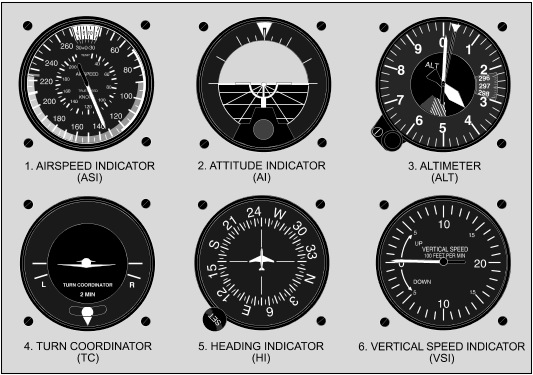
\includegraphics[width=0.9\textwidth]{imagenes/1.3.distribucion.normalizada.instrumental.en.tablero/6_pack.png}

\end{frame}

\begin{frame}{Distribuci\'on Normalizada del Instrumental en el
 Tablero}
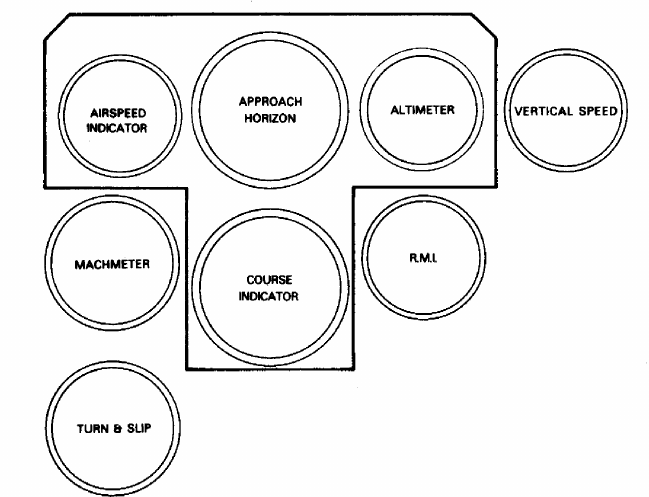
\includegraphics[width=0.9\textwidth]{imagenes/1.3.distribucion.normalizada.instrumental.en.tablero/6.png}

\end{frame}

\begin{frame}{Distribuci\'on Normalizada del Instrumental en el
 Tablero}
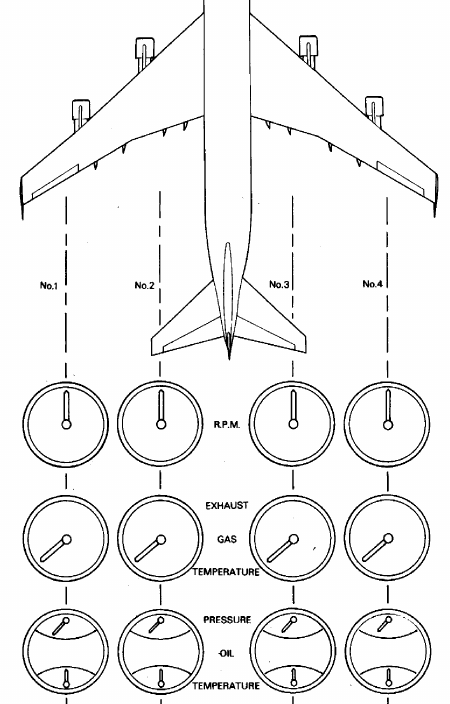
\includegraphics[width=0.4\textwidth]{imagenes/1.3.distribucion.normalizada.instrumental.en.tablero/instrumentos_motor.png}
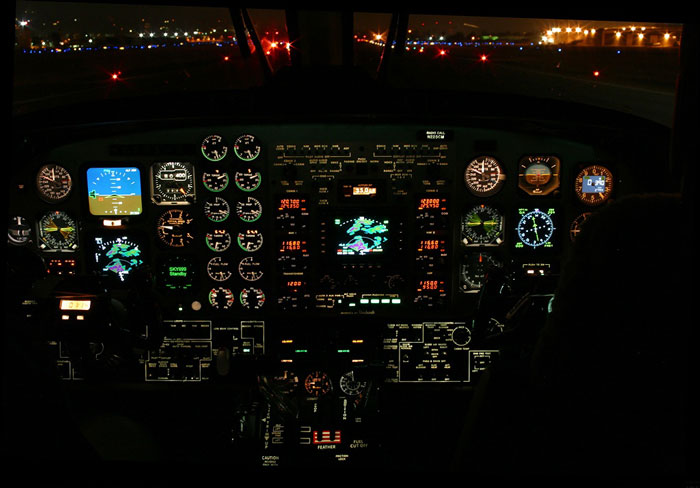
\includegraphics[width=0.6\textwidth]{imagenes/1.3.distribucion.normalizada.instrumental.en.tablero/iluminacion.jpg}

\end{frame}




\subsection{Presentaci\'on en Pantalla Electr\'onica}
\label{sec:cap.1.4.presentacion.en.pantalla.electronica}

%	1.4. Presentacion en Pantalla Electronica.
%	version 2018


\begin{frame}
  \begin{columns}
    \begin{column}{0.5\textwidth}
      \begin{block}{Un poco de historia...}
{\normalsize
        \begin{description}
        \item[1970] NASA investigaci\'on en como mostrar instrumentos
          de vuelo
        \item[1982]Boeing 767 con pantallas electr\'onicas de datos tipo \ac{CRT}
        \item[1990]Fines de la d\'ecada, pantallas \ac{LCD} reemplazan
          pantallas \ac{CRT}
        \item[Actualidad] La mayor\'ia de las aeronaves equipadas con
          pantallas \ac{LCD}
        \item[Futuro] Uso de pantallas tipo \ac{OLED}
        \end{description}
}
      \end{block}
    \end{column}

    \begin{column}{0.5\textwidth}
  \includegraphics[width=0.9\linewidth]{imagenes/1.4.pantalla.electronica/CRT.gif}

\vspace{3mm}

  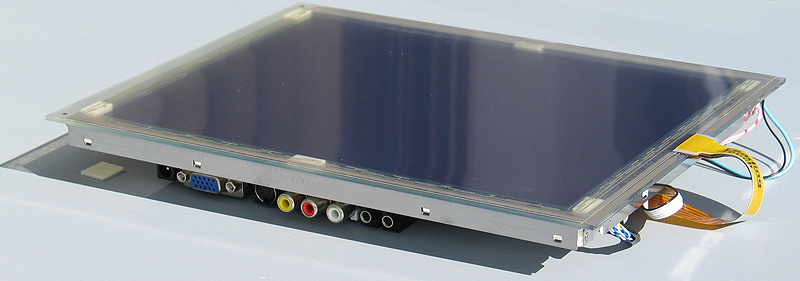
\includegraphics[width=0.8\linewidth]{imagenes/1.4.pantalla.electronica/LCD.jpg}

\vspace{3mm}

  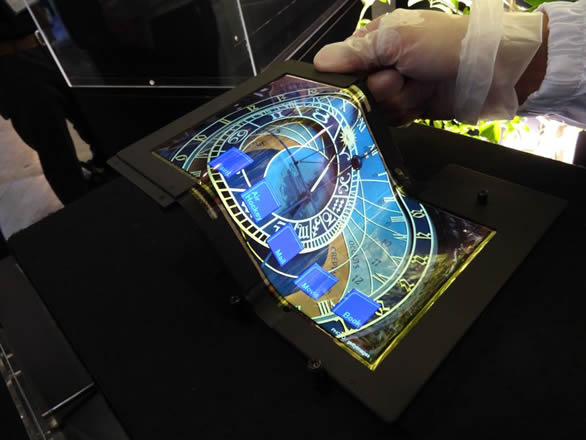
\includegraphics[width=0.7\linewidth]{imagenes/1.4.pantalla.electronica/foldable-oled-display.jpg}
    \end{column}
  \end{columns}

\end{frame}

\begin{frame}

  \begin{block}{ EIS (Electronic Instrument
      System)}

Ejemplos:

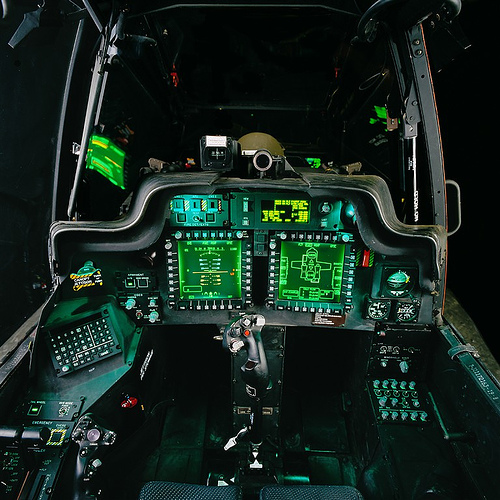
\includegraphics[width=0.34\textwidth]{imagenes/1.4.pantalla.electronica/apache.jpg}
\hspace{3mm}
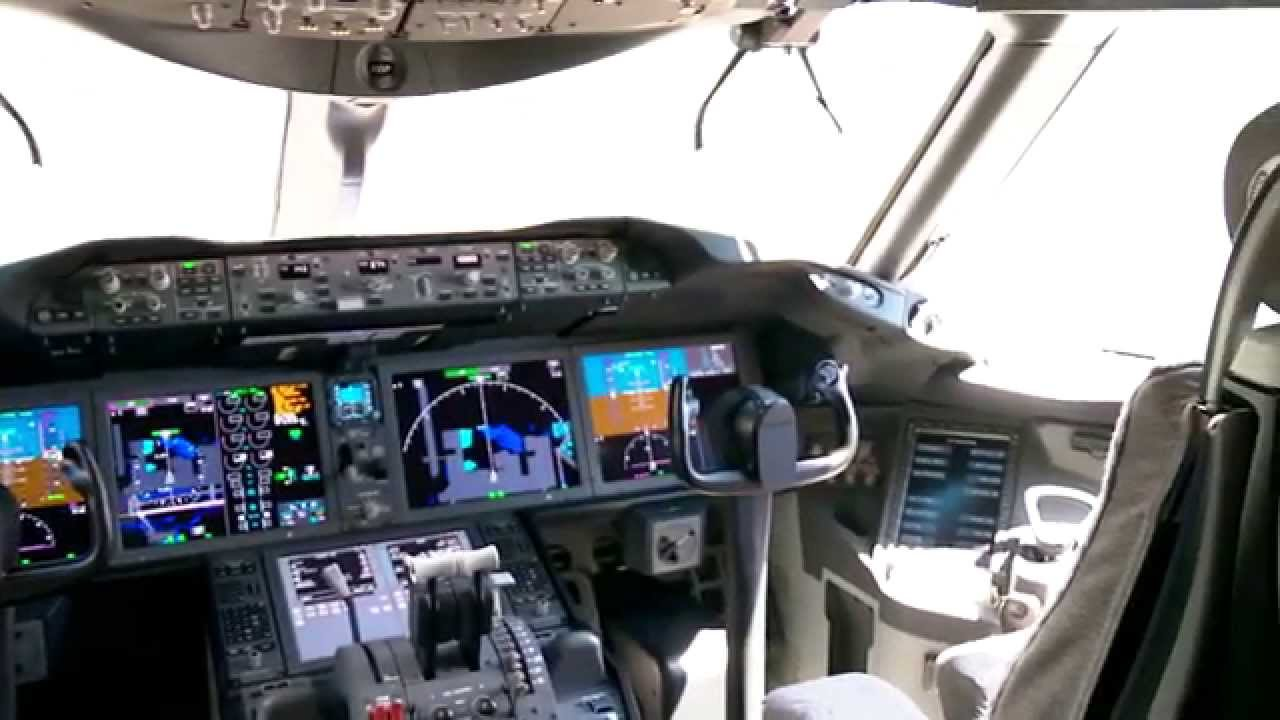
\includegraphics[width=0.55\textwidth]{imagenes/1.4.pantalla.electronica/dreamliner.jpg}

Helic\'optero Apache \hspace{25mm} Boeing 787 Dreamliner
  \end{block}

\end{frame}

\begin{frame}
  Una instalaci\'on EIS sigue la secuencia siguiente:

\vspace{3mm}


 Pantallas \qquad $\Longrightarrow$ \qquad
 Controles  \qquad $\Longrightarrow$ \qquad
 Procesadores de datos 

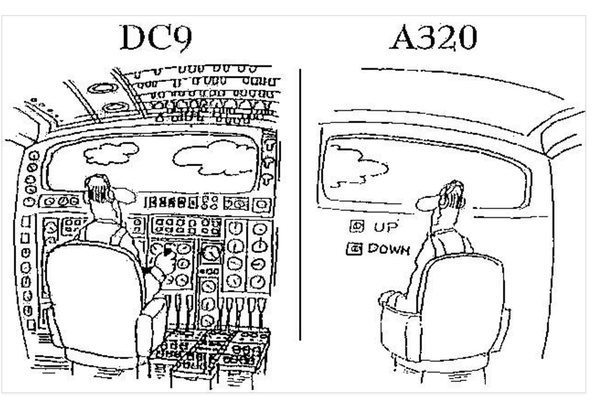
\includegraphics[width=0.85\textwidth]{imagenes/1.4.pantalla.electronica/efis_humor.png}

\end{frame}

\begin{frame}

  \begin{block}{Bus de datos}
{\small
    Las se\~nales que se env\'ian entre los distintos componentes del
    EIS se transmiten por una l\'inea de transmisi\'on digital
    denominada ``{\it Bus de Datos}". Las se\~nales transmitidas son
    peque\~nos pulsos de tensi\'on en c\'odigo binario (unos y
    ceros). Seg\'un el protocolo los unos y ceros se diferencian por
    tener valores distintos de tensiones positivas o negativas,
    variaciones de tensiones ascendentes o descendentes, falta de
    tensi\'on, etc. Los pusos de tensi\'on tienen duraciones
    extremadamente breves a fin de enviar una gran cantidad de
    informaci\'on en poco tiempo.
}
  \end{block}


  \begin{columns}
    \begin{column}{0.5\textwidth}
      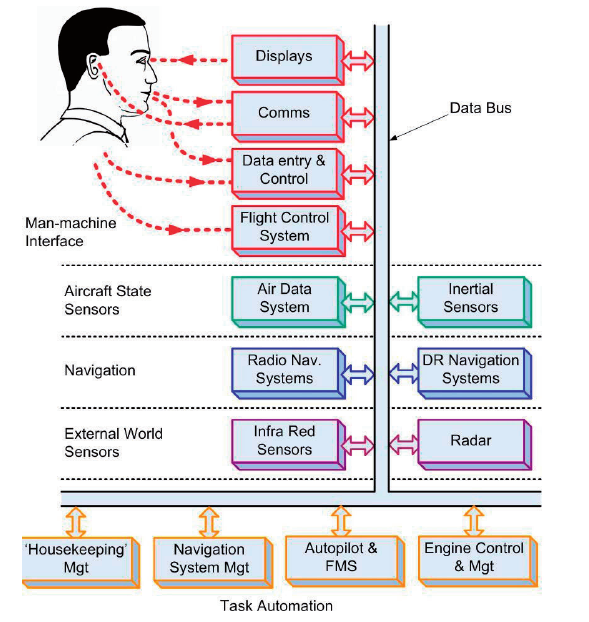
\includegraphics[width=\linewidth]{imagenes/1.2.clasificacion.instrumentos/tipos_instrumentos.png}

      {\tiny Referencia: \cite{Introduction_to_Avionics_Systems}}
    \end{column}
  \begin{column}{0.5\textwidth}
    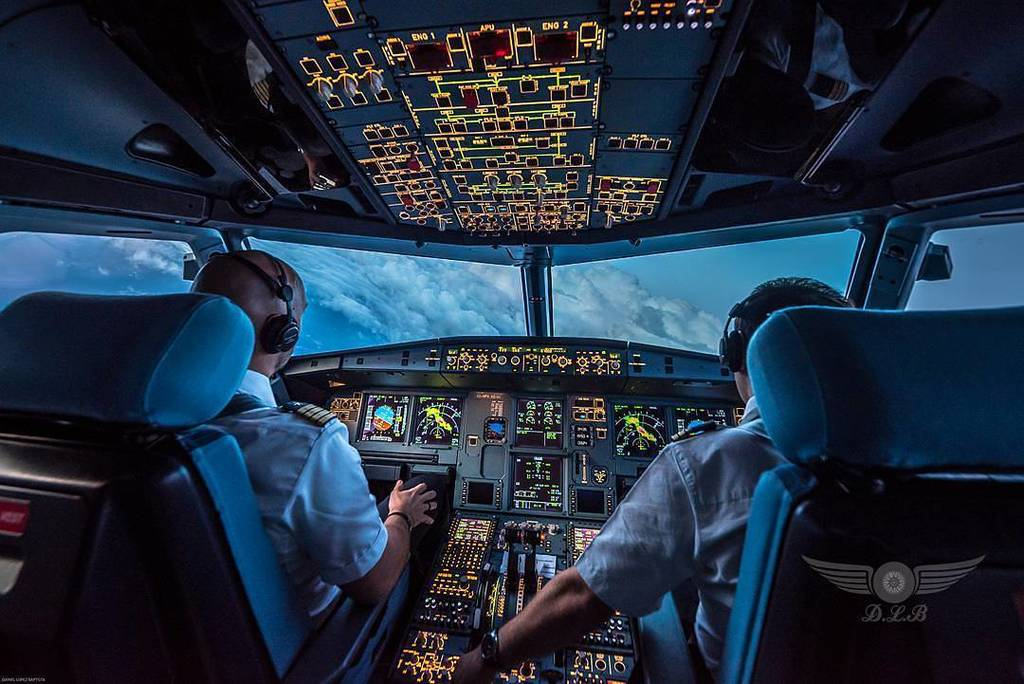
\includegraphics[width=\linewidth]{imagenes/1.2.clasificacion.instrumentos/glass_cockpit.jpg}
%    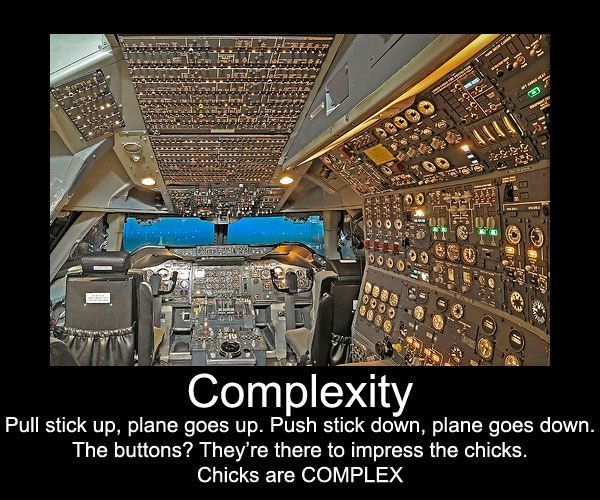
\includegraphics[width=\linewidth]{imagenes/1.2.clasificacion.instrumentos/humor_complejidad.jpg}
  \end{column}
  \end{columns}

\end{frame}

\begin{frame}

% Mientras que en el sistema de numeración decimal se usan diez dígitos (diez símbolos), en el binario se usan solo dos dígitos, el 0 y el 1. Un bit o dígito binario puede representar uno de esos dos valores: 0 o 1. 

% El bit es la unidad mínima de información empleada en informática, en cualquier dispositivo digital, o en la teoría de la información.

  \begin{exampleblock}{Buses de datos}
    \begin{itemize}
    \item Un sistema digital t\'ipico puede enviar se\~nales de pulsos
      con duraciones de 10 $\mu$seg

    \item Un sistema de bus digital usual en avi\'onica es el
      ARINC (Aeronautical Radio INCorporated), bajo cuya denominaci\'on existen una gran cantidad
      de protocolos de comunicaciones con diferencias b\'asicas en los
      par\'ametros de transmisi\'on y recepci\'on.

    \item ARINC es una gran empresa que desarrolla y opera
      sistemas y servicios para garantizar la eficiencia, el
      funcionamiento y el rendimiento de la aviaci\'on y la industria
      del transporte. Fue fundada en 1929 por cuatro grandes
      aerol\'ineas para proporcionar un \'unico licenciatario de
      comunicaciones fuera del gobierno.

    \item Por ejemplo, el ARINC 429 es una especificaci\'on que define
      como los equipos y sistemas de avi\'onica deber\'ian comunicarse
      entre s\'i. Emplea una transmisi\'on unidireccional conocida
      como Mark 33 DITS, de palabras de 32 bits a trav\'es de un
      par trenzado usando el formato bipolar RZ. Los mensajes se
      transmiten a una tasa de 12,5 o 100 kilobits por segundo. La
      transmisi\'on y la recepci\'on se realizan en puertos separados,
      por lo que es posible que se necesiten muchos cables en las
      aeronaves que utilizan una gran cantidad de sistemas de
      avi\'onica.
    \end{itemize}
  \end{exampleblock}

\end{frame}

\begin{frame}

  \begin{block}{Pantallas presentaci\'on de datos}

    \begin{itemize}
      \begin{multicols}{3}
      \item \ac{CRT}
      \item \ac{LCD}
      \item \ac{OLED}
      \end{multicols}
    \end{itemize}

	La imagen se forma por la uni\'on de muchos puntos (p\'ixeles). El p\'ixel es la menor 
unidad homog\'enea en color que forma parte de una imagen digital. 

      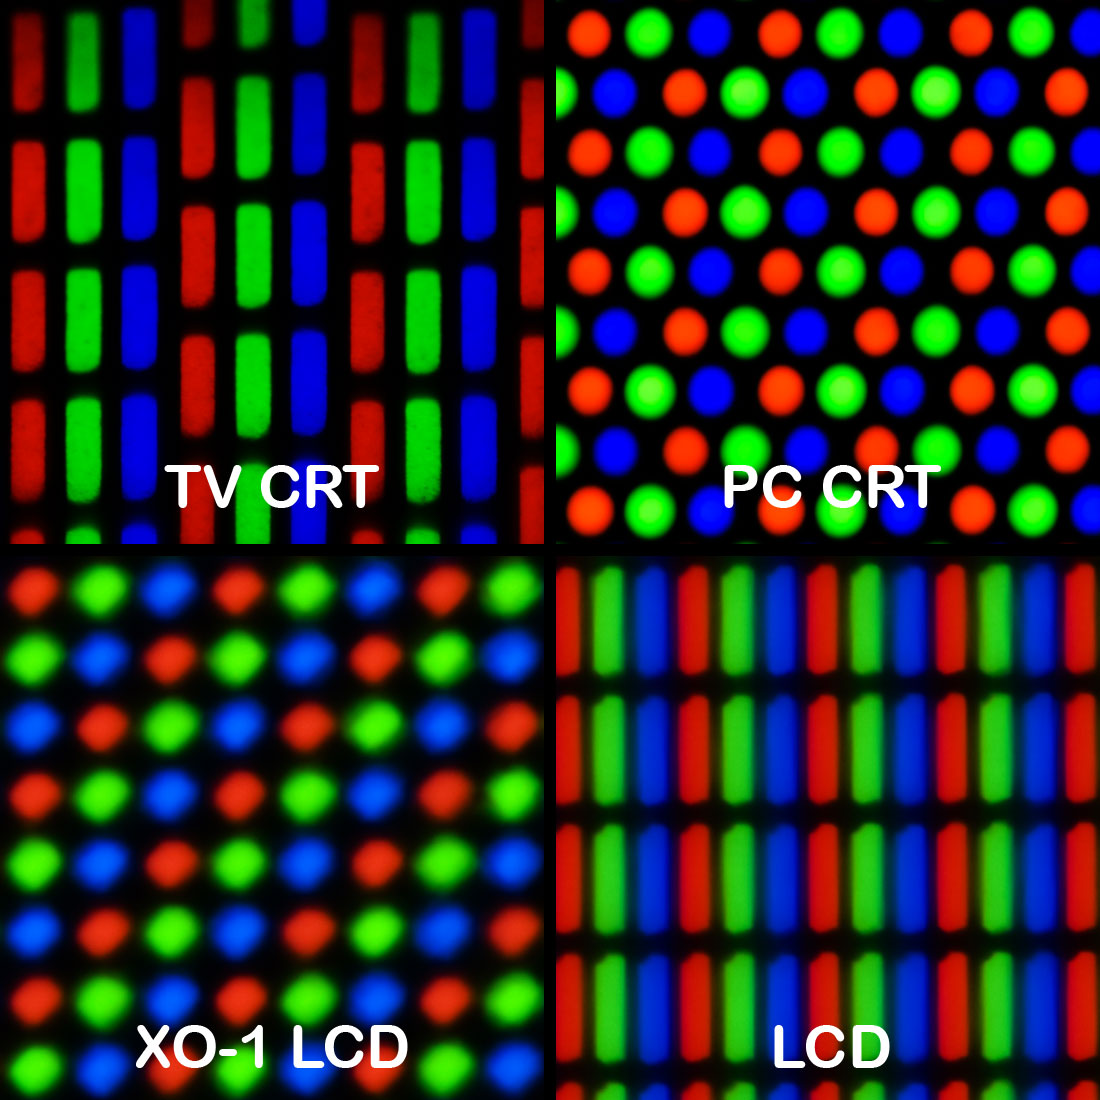
\includegraphics[width=0.4\linewidth]{imagenes/1.4.pantalla.electronica/Pixel_geometry_01_Pengo.jpg}


  \end{block}
  
\end{frame}

\begin{frame}

  \begin{block}{Pantalla \ac{CRT}}
    \begin{columns}[T]

      \begin{column}[T]{0.6\textwidth}
        \includegraphics[width=\linewidth]{imagenes/1.4.pantalla.electronica/CRT.gif}
      \end{column}

      \begin{column}[T]{0.4\textwidth}
	
        \begin{itemize}
{\footnotesize
        \item Los datos son enviados desde la computadora por medio
          del puerto de video hacia los circuitos del monitor.

        \item           Los circuitos internos los reciben y de acuerdo a lo
          especificado por la computadora controla los ca\~nones de
          electrones.

        \item           Estos ca\~nones lanzan haces electrones hacia la pantalla, la
          cu\'al tiene zonas sensibles fosforescentes (p\'ixeles) y al
          recibirlos emiten un peque\~no pulso de luz.

}
        \end{itemize}


      \end{column}
    \end{columns}

    \begin{itemize}
 {\footnotesize 
        \item           Para pantallas monocrom\'aticas integra solo un ca\~n\'on, para el
          monitor a color integra tres ca\~nones y cada uno controla un
          color (rojo, verde y azul), sistema RGB, los cuales
          mezclados determinan el color del p\'ixel en pantalla.

        \item           La trayectoria de los electrones en sentido vertical y
          horizontal hacia los p\'ixeles de la pantalla, es controlada
          por medio bobinas que emiten de campos magn\'eticos.

        \item           Como el tiempo que permanece encendido el p\'ixel es muy
          corto, el proceso se repite varias veces por segundo en toda
          la pantalla de manera horizontal y hacia abajo (entre 56 y
          120 veces); a este proceso se le denomina frecuencia y se
          mide en Hz o ciclos sobre segundo.

        \item           Lo anterior se repite aunque para el usuario la pantalla
          parezca est\'atica, \'esta se esta refrescando varias veces por
          segundo.
}
    \end{itemize}

  \end{block}
\end{frame}


\begin{frame}

  \begin{block}{Pantalla \ac{LCD}}
    \begin{columns}[T]

      \begin{column}[T]{0.5\textwidth}
        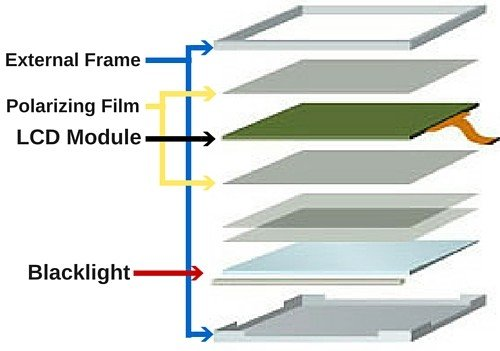
\includegraphics[width=\linewidth]{imagenes/1.4.pantalla.electronica/lcd_partes.jpg}
      \end{column}

      \begin{column}[T]{0.5\textwidth}
	
        \begin{itemize}
{\footnotesize
        \item Este dispositivo cuenta con un microprocesador encargado de determinar la posici\'on de cada píxel.

        \item Una pantalla LCD cuenta con 2 placas de vidrio, una de ellas esta iluminada de la parte trasera por una luz intensa procedente de l\'amparas CCFL (Cold-Cathode Fluorescent Lamps / L\'amparas fluorescentes de c\'atodo fr\'io), lo que permite el brillo en la pantalla.

        \item Una vez que se determina el p\'ixel a colorear, la celda cuenta con 3 sustancias propensas a recibir corriente y colorearse de alg\'un color básico (verde, rojo y azul) por medio de polarizaci\'on.

        \item La corriente que le llega a cada p\'ixel determina la saturaci\'on para cada color y as\'i se genera la gama de colores.

        \item El proceso se repite cada vez que cambian las im\'agenes en la pantalla.
	}
        \end{itemize}


      \end{column}
    \end{columns}

    \begin{itemize}
 {\footnotesize 
        \item           
	}
    \end{itemize}

  \end{block}
\end{frame}


\begin{frame}

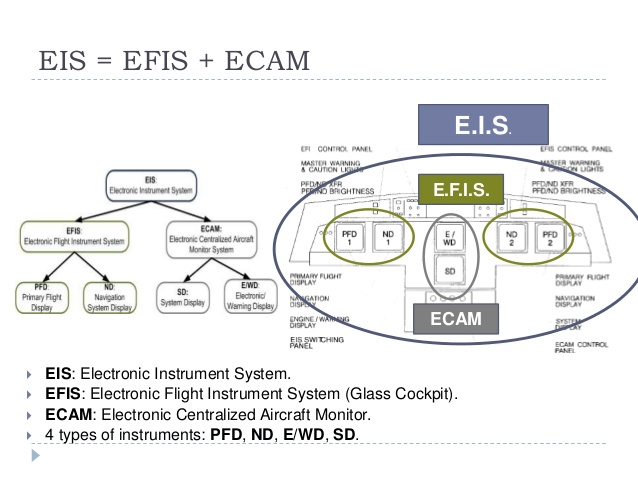
\includegraphics[width=0.85\textwidth]{imagenes/1.4.pantalla.electronica/efis.jpg}

\end{frame}

% \begin{frame}
  
%   \begin{bclogo}[couleur=blue!10, arrondi = 0.1,
% 	logo = \bccrayon, ombre = true
% 	]{Bclogo parece versatil}

% 	Box de prueba con bclogo
    
%   \end{bclogo}


% \end{frame}



\begin{frame}

     \begin{block}{ PFD: Primary Flight Display}
{\footnotesize
	% Presenta los siguientes instrumentos
	
	%  Airspeed Indicator, 
	%  Altimeter, 
	%  HSI (Horizontal Situation Indicator),
	%  VSI (Vertical Speed Indicator)
	

	El PFD reemplaza a los seis (6) instrumentos tradicionales

	Muestra la informaci\'on cr\'itica de vuelo 
	incluyendo velocidad, altitud,direcci\'on (heading)
	actitud y velocidad vertical

	Est\'a dise\~nado para mejorar las alertas al piloto
	al integrar informaci\'on en una sola pantalla

	Reduce el tiempo para monitorear otros instrumentos

	Alerta a los pilotos de condiciones potencialmente peligrosas
        cambiando el color o la forma en el display o mediante alertas
        de sonido. (baja velocidad, alta tasa de descenso) 
}
    \end{block}

 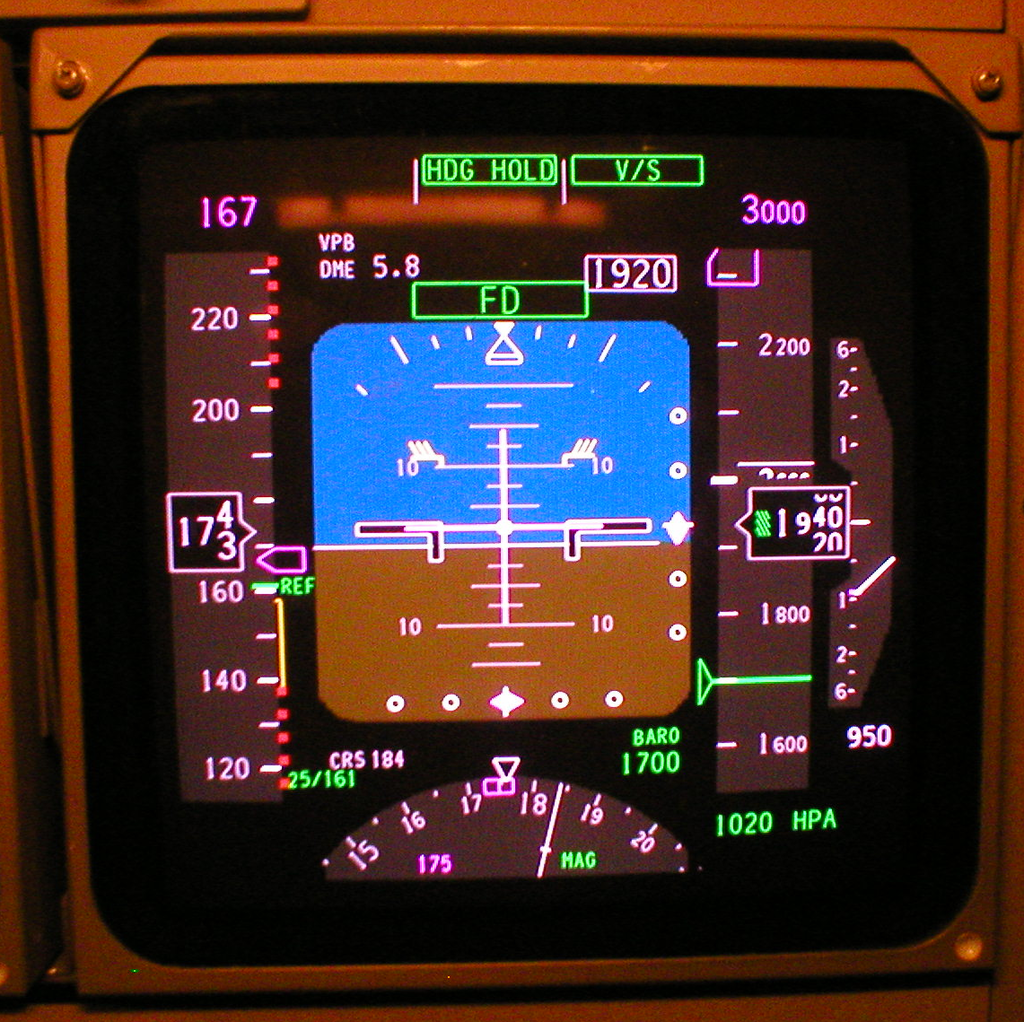
\includegraphics[width=3cm]{imagenes/1.4.pantalla.electronica/Primary_Flight_Display,_Boeing_747-400.png}\\
 

    \end{frame}      
    
\begin{frame}

  \begin{block}{ MDF: MultiFunction Display o ND (Navigation Display)}

    Informaci\'on para navegaci\'on (VOR, DME, ILS)

    Informaci\'on clim\'atica de m\'ultiples sistemas (radar a bordo,
    sensores de detecci\'on de rel\'ampagos)

    Idem al PFD el MDF puede cambiar color, forma y dar alertas
    sonoras

    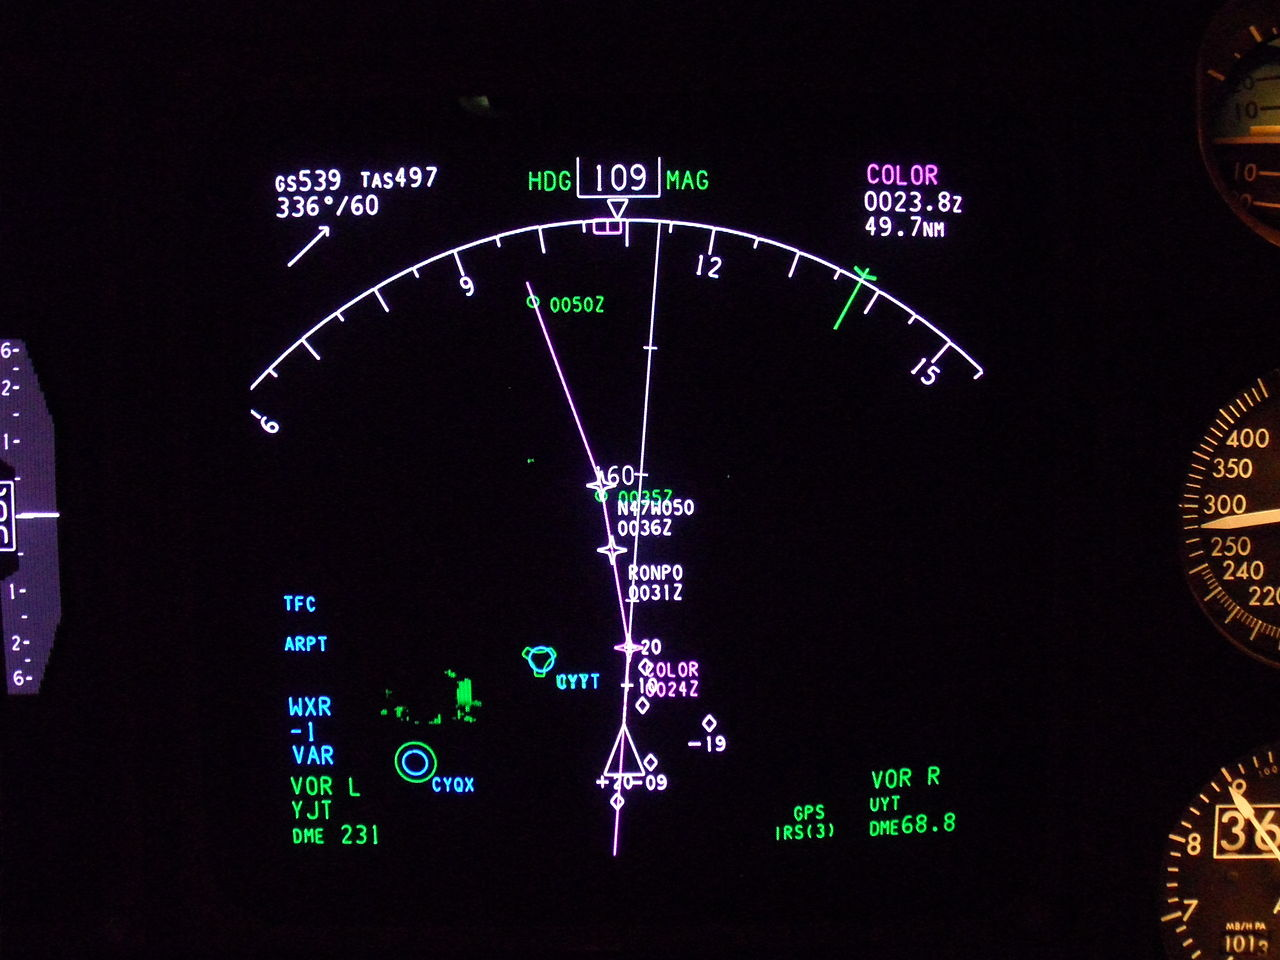
\includegraphics[width=6cm]{imagenes/1.4.pantalla.electronica/Navigation_Display_(ND)_on_Boeing_747-400.jpg}
  \end{block}
    \end{frame}      
    
\begin{frame}

  \begin{block}{ ECAM : Electronic Centralized Aircraft Monitor
    (Airbus) \\
     EICAS : Electronic Centralized Aircraft Monitor (Boeing)}


    Monitorear los sistemas de la aeronave: p.e. combustible, sistemas
    el\'ectricos y del motor

    Usualmente dos (2) pantallas, una arriba de la otra

    La pantalla superior muestra sistemas motores, posici\'on flaps
    cantidad de combustible e informaci\'on de alerta

    La pantalla inferior muestra diversos par\'ametros de sistemas

    Brinda alarmas en caso de malfuncionamiento

    P.e. en caso de p\'erdida de presi\'on de aceite en un motor, el
    ECAM hace sonar una alerta, cambia la pantalla a una que muestra
    el sistema de aceite y se\~nala la baja presi\'on con una caja
    roja.

  \end{block}
    \end{frame}

\begin{frame}
  \begin{tabular}{ccc}
	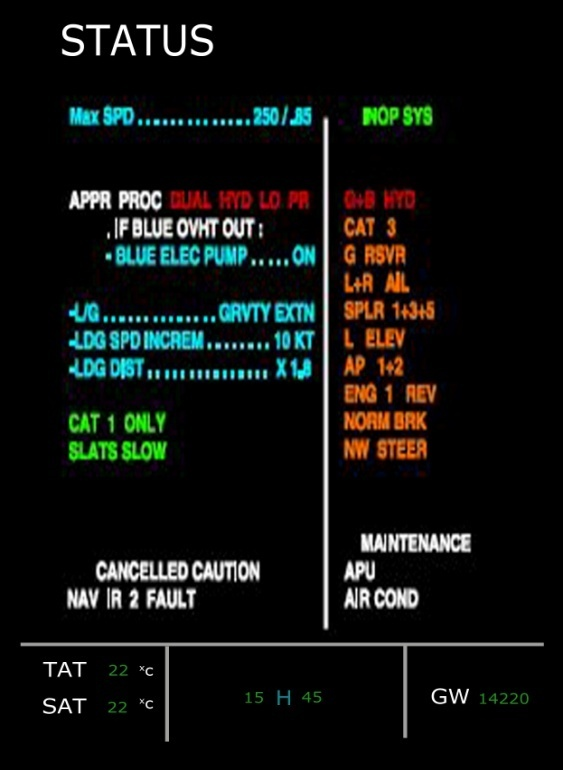
\includegraphics[width=4.5cm]{imagenes/1.4.pantalla.electronica/eicas_status.jpg}
	& \hspace{3mm} &
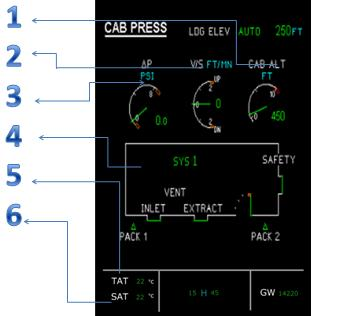
\includegraphics[width=6cm]{imagenes/1.4.pantalla.electronica/eicas_presion_cabina.jpg}
	\\
   	EICAS status & 
	& EICAS presi\'on cabina.  
% \parbox{\linewidth}{\tiny 1. Cabin altitude (height),
% 2. Vertical Speed (height/min),
% 3. Pressure,
% 4. Cabin,
% 5. True air temperature}
	\\
\end{tabular}

\end{frame}


\begin{frame}
  \begin{center}
    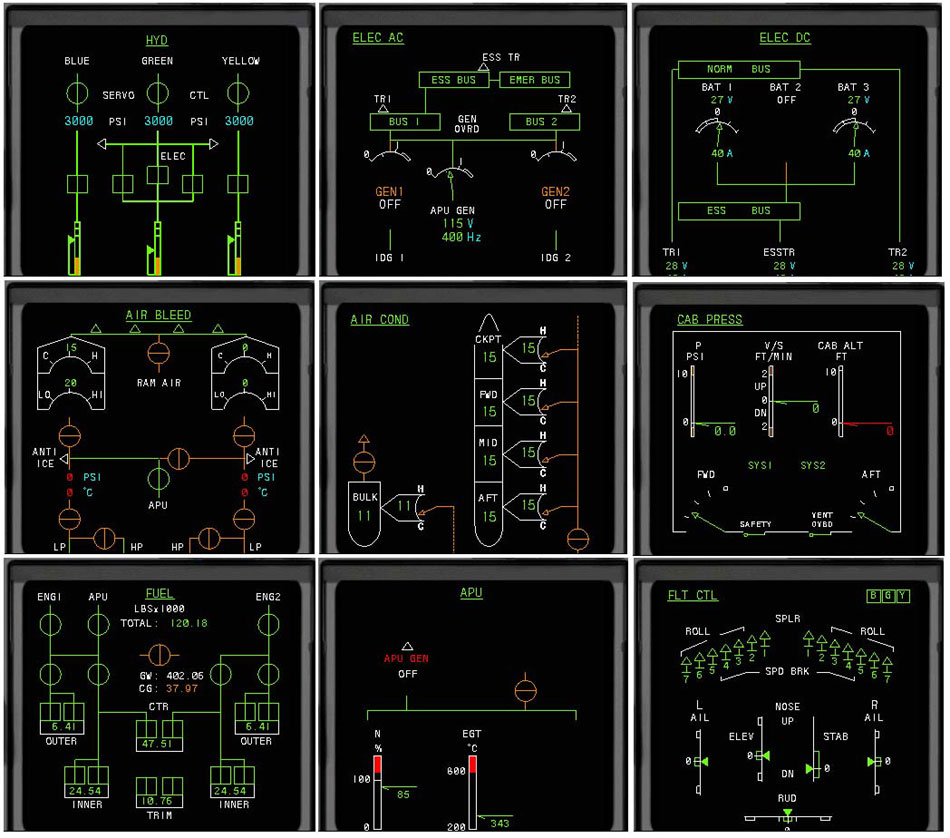
\includegraphics[width=0.65\textwidth]{imagenes/1.4.pantalla.electronica/ecam_airbus.jpg}

    \vspace{3mm}

    ECAM presentaci\'on
  \end{center}
\end{frame}

\begin{frame}

  \begin{block} { \ac{FMS}
%: Flight Management System
}

    Instrumentos para mantener el plan de vuelo (flight plan) permite
    a los pilotos modificarlo en vuelo

    Dada la posici\'on y el plan de vuelo, el  \ac{FMS} se encarga de guiar
    el avi\'on a lo largo del mismo, gestiona los diversos factores
    que afectan al vuelo del avi\'on, tanto la ruta que tiene que
    seguir, como los niveles \'optimos a los cuales volar para reducir
    el consumo y hacer un vuelo m\'as eficiente.


    Usualmente se presenta como una pantalla peque\~na y un teclado

    El \ac{FMS} se compone principalmente del \ac{CDU} y 
    el \ac{FMC}
  \end{block}


% {\bf Autopiloto (AP)}

% 	Computadora que permite que una aeronave se vuele a s\'i misma.

% 	Se utiliza habitualmente en vuelos de larga duraci\'on

% 	El piloto se encuentra presente siempre para monitorear
% 	y chequear que el vuelo se desarrolle seg\'un el plan


% \end{itemize}

\end{frame}

\begin{frame}


El piloto introduce los datos al \ac{FMC} a trav\'es de la \ac{CDU} que no es m\'as que un teclado 
y una pantalla que sirve para la comunicaci\'on entre el piloto y el \ac{FMC}. 
A trav\'es de la \ac{CDU} el piloto programa la ruta del vuelo, las \ac{SID}  
y las \ac{STAR}, as\'i como los puntos en las rutas donde el avi\'on debe ascender 
a niveles \'optimos seg\'un disminuye el peso del avi\'on.

    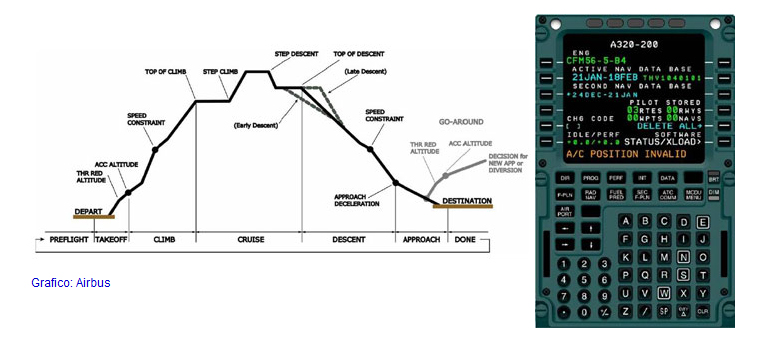
\includegraphics[width=0.9\textwidth]{imagenes/1.4.pantalla.electronica/fms_plan_vuelo.jpg}
  \end{frame}
  

\begin{frame}{Presentaci\'on en Pantalla Electr\'onica}
{\small
El \ac{FMC} adem\'as adquiere datos de muchos de los sistemas del avi\'on. Para empezar recibe informaci\'on de los inerciales, y de los \ac{GPS} para triangular la posici\'on del avi\'on y tener una posici\'on a\'un m\'as exacta de donde se encuentra el avi\'on.

El \ac{FMS} tiene principalmente dos bases de datos. Una base de datos de navegaci\'on, donde est\'an almacenadas las rutas, aerov\'ias, \ac{SID}, \ac{STARS}, as\'i como las frecuencias de las radio ayudas a la navegaci\'on que va a sintonizar autom\'aticamente a lo largo de la ruta. Esta base de datos se renueva cada 28 d\'ias para poder estar actualizada cuando se producen cambios en los espacios a\'ereos o se modifican procedimientos de aproximaci\'on. 
El \ac{FMC} es capaz de guardar dos (2)  bases de datos de navegaci\'on.

La otra base de datos es de performance del avi\'on. Esta base de datos contiene informaci\'on de los niveles \'optimos de vuelo dependiendo del peso del avi\'on. Los consumos que tiene el avi\'on para cada peso y nivel de vuelo. Las predicciones de ascenso y descenso del avi\'on.

Como el avi\'on va envejeciendo a lo largo de su vida y disminuyendo sus performance, el \ac{FMS} admite un valor de degradaci\'on de las performance que se introduce en la p\'agina principal del \ac{CDU} para que de unas previsiones de combustibles m\'as reales seg\'un el avi\'on se va haciendo ``mayor''
}
\end{frame}


\begin{frame}

{\small
Con el tiempo el \ac{FMS} ha ido mejorando y abarcando nuevas posibilidades. As\'i Airbus cambia el nombre 
al \ac{CDU} y le ha pasado a llamar \ac{MCDU}. Ahora no solamente se puede acceder 
al \ac{FMC} a trav\'es del teclado de la \ac{CDU} si no a una infinidad de nuevos servicios.

Mediante el \ac{MCDU} se accede al \ac{ATSU}, \ac{AIDS}, \ac{CFDS} y al \ac{FMS} 
comentado hasta ahora y llamado por Airbus \ac{FMGS}.

\begin{itemize}
\item El \ac{ATSU} es el acceso al Acars o sistema de comunicaciones
  tanto con la compa\~n\'ia como con el control a\'ereo. A trav\'es de
  esta opci\'on se recibe desde la hoja de carga, cualquier mensaje
  escrito que envie la compa\~n\'ia, hasta la autorizaci\'on para
  ingresar a otro pa\'is.

\item   El \ac{CFDS} es usado principalmente por el personal de
  mantenimiento.  En el est\'an los reportes de mantenimiento del
  vuelo, y las aver\'ias que haya tenido el avi\'on, por muy
  peque\~nas o temporales que hayan sido (aunque haya sido un fallo
  temporal de cualquier fusible por menos de 1 sg se queda
  registrado).

\item   El \ac{AIDS} es otra herramienta que maneja mantenimiento, sirve
  para interrogar y realizar TEST a cualquier sistema del avi\'on para
  conocer en qu\'e estado de operatividad se encuentra.
\end{itemize}


}
\end{frame}

\begin{frame}

    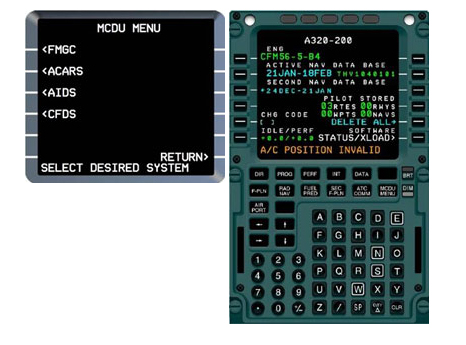
\includegraphics[width=0.9\textwidth]{imagenes/1.4.pantalla.electronica/mcdu.jpg}

\end{frame}

\begin{frame}
  
Las pantallas \ac{OLED} consisten en paneles muy delgados que permiten un ahorro
de peso y espacio, la potencia que necesitan es muy reducida y poseen posibilidades
de emplearse como pantallas flexibles aunque, tambi\'en poseen limitaciones.
El principal problema es la madurez de la tecnolog\'ia que no es suficiente
para el uso en avi\'onica, su brillo no es suficiente y su vida \'util, reducida.




\url{http://www.optinvent.com/wp-content/uploads/2016/03/Odicis_IDW10final_2.pdf}

\end{frame}

% %-----------------acronimos

\section{Acr\'onimos}
\label{sec:acronimos}

%****** Acronyms and abbreviations in avionics ******
%***** [edit] A *****

% \acrodef{AGPL}{Affero General Public License}
% AGPL: Affero General Public License.




%     * ACARS: Aircraft Communications Addressing and Reporting System
%     * ACAS: Airborne Collision Avoidance System
%     * ACP: Audio control panel
%     * ACS: Audio control system
%     * ADAHRS: Air data and attitude heading reference system
%     * ADC: Air data computer
%     * ABAS: Aircraft-based augmentation system
%     * ADF: Automatic direction finder
%     * ADI: Attitude director indicator
%     * ADIRS: Air Data Inertial Reference System
%     * ADIRU: Air data inertial reference unit
%     * ADM: Air data module
%     * ADS: Either; Automatic Dependent Surveillance or air data system
%     * ADS-A: Automatic Dependent Surveillance-Address
%     * ADS-B: Automatic Dependent Surveillance-Broadcast
%     * AFCS: Automatic flight control system
%     * AFD: Autopilot flight director
%     * AFDC: Autopilot flight director computer
%     * AFDS: Autopilot flight director system
%     * AFIS: Either; Automatic flight information service or airborne flight
%       information system
%     * AGACS: Automatic ground–air communications system, is also known as ATCSS
%       or data link
%     * AGDL: Air-Ground Data Link
%     * AGC: Automatic gain control
%     * AHC: Attitude heading control
%     * AHRS: Attitude and Heading Reference Systems

\acrodef{AIDS}{Aircraft Integrated Data System}
      AIDS: Aircraft Integrated Data System

%     * ALC: Automatic level control
%     * ALT: Either; altimeter or altitude
%     * ALT Hold: altitude hold mode
%     * ALTS: Altitude select
%     * AMLCD: Active-matrix liquid crystal display
%     * ANC: Active noise cancellation
%     * ANN: Annunciator – caution warning system normally containing visual and
%       audio alerts to the pilot
%     * ANR: Active noise reduction
%     * ANT: Antenna
%     * A/P: Autopilot
%     * APC: Autopilot computer
%     * APS: Autopilot system
%     * APU: Auxiliary power unit
\acrodef{ARINC}{Aeronautical Radio INCorporated}
	ARINC: Aeronautical Radio INCorporated 

%     * ASD: Aircraft situation display
%     * ASDL: Aeronautical satellite data link
%     * ASR: Airport surveillance radar
%     * ASU: Avionics switching unit
\acrodef{ATC}{Air traffic control} ATC: Air traffic control
%     * ATCRBS: Air Traffic Control Radar Beacon System
%     * ATCSS: Air traffic control signaling system
%     * ATI: Unit of measure for instrument size, a standard 3¨û cutout is a 3ATI
%     * ATM: Air traffic management

\acrodef{ATSU}{Air Traffic Services Unit}
	ATSU: Air Traffic Services Unit%, implementada por AIRBUS en sus aviones (no en los A300/310), 
%		realiza las funciones generalmente usuales en unidades de gesti\'on de comunicaciones
%		de otro tipo de aviones.

%     * Avionics: Aviation + electronics
%     * AWG: American wire gauge


% ***** [edit] B *****
%     * B RNAV: Basic area navigation
%     * BARO: Barometric indication, setting or pressure
%     * BCRS: Back course
%     * BDI: Bearing distance indicator
%     * BGAN: Broadcast Global Area Network
\acrodef{BIT}{BInary Digit}
	BIT: BInary Digit

% ***** [edit] C *****
%     * CAI: Caution annunciator indicator
%     * CAT I: Operational performance Category 1
%     * CAT I Enhanced Allows for lower minimums than CAT I in some cases to CAT
%       2 minimums
%     * CAT II: Operational performance Category II
%     * CAT IIIa: Operational performance Category IIIa
%     * CAT IIIb: Operational performance Category IIIb
%     * CAT IIIc: Operational performance Category IIIc
%     * CODEC: Coder/decoder
%     * CDI: Course deviation indicator
%     * CDTI: Cockpit display of traffic information

\acrodef{CFDS}{Centralised Fault Display System}
	CFDS: Centralised Fault Display System

%     * CFIT: Controlled flight into terrain

\acrodef{CDU}{Control Display Unit}
	CDU: Control Display Unit

%     * COMM or COM: Communications receiver
%     * CNS: Communication, navigation, surveillance
%     * CNS/ATM: Communication, navigation, surveillance/air traffic Management
%       [1]
%     * CPDLC: Controller–pilot data link communications
%     * CPS: Cycles per second
%     * CRT: Cathode ray tube
\acrodef{CRT}{Cathode Ray Tube}
	CRT: Cathode Ray Tube
%     * CTAF: Common traffic advisory frequency
%     * CV/DFDR: Cockpit voice and digital flight data recorder
%     * CVR: Cockpit voice recorder
%     * CWS: Control wheel steering
% ***** [edit] D *****
%     * DA: Drift angle
%     * DAPs: Downlink of aircraft parameters
%     * DCDU: Data link control and display unit
%     * DG: Directional gyroscope
%     * DGPS: Differential global positioning system
%     * DH: Decision height
\acrodef{DITS}{Digital Information Transfer System}
	DITS: Digital Information Transfer System
%     * DLR: Data link recorder
%     * DME: Distance measuring equipment
%     * DNC: Direct noise canceling
%     * DP: Departure procedures
%     * DSP: Digital signal processing
%     * DUAT: Direct user access terminal
% ***** [edit] E *****
%     * EADI: Electronic attitude director indicator

\acrodef{EFD}{Electronic flight display}
      EFD: Electronic flight display

%     * EFIS: Electronic flight instrument system
%     * EGPWS: Enhanced ground proximity warning system
%     * EGT: Exhaust gas temperature
%     * EHS: Enhanced surveillance
%     * EHSI: Electronic horizontal situation indicator

\acrodef{EICAS}{Engine indication crew alerting system}
      EICAS: Engine indication crew alerting system

%     * ELT: Emergency locator transmitter
%     * ENC: Electronic noise canceling
%     * ENG: Engine
%     * ENR: Electronic noise reduction
%     * EPR: Engine pressure ratio
%     * ETOP: Extended-range twin-engine operation
% ***** [edit] F *****
%     * FADEC: Full authority digital engine control
%     * FANS: Future Air Navigation System
%     * FAT: Free air temperature
%     * FDPS: Flight plan Data Processing System
%     * FDRS: Flight data recorder system
%     * FDU: Flux detector unit
%     * FF: Fuel flow
%     * FIS-B: Flight information services – broadcast
%     * FLIR: Forward-looking infra-red
%     * FLTA: Forward-looking terrain avoidance

\acrodef{FMC}{Flight Management Computer}
	FMC: Flight Management Computer

\acrodef{FMGS}{Flight Management Guidance System}
	FMGS: Flight Management Guidance System

\acrodef{FMS}{Flight Management System}
      FMS: Flight Management System

%     * FREQ: Frequency
%     * FSS: Flight service station
%     * FWS: Flight warning system
%     * FYDS: Flight director/ Yaw damper system

% ***** [edit] G *****

%     * GBAS: Ground based augmentation system
%     * GCAS: Ground collision avoidance system
%     * GCU: Generator control unit
%     * GDOP: Geometric dilution of precision
%     * GGS: Global positioning system ground station
%     * GHz: Gigahertz
%     * GLNS: GPS Landing and Navigation System
%     * GLNU: GPS landing and navigation unit
%     * GLONASS: Global Navigation Satellite System
%     * GLS: GPS Landing System
%     * GLU: GPS landing unit

\acrodef{GND}{Ground}
	GND: Ground (tierra)


    % * GNSS: Global Navigation Satellite System
    % * GMT: Greenwich Mean Time

\acrodef{GPS}{Global Positioning Satellite or Global Positioning System}
    GPS: Global Positioning Satellite or Global Positioning System

    % * GPWC: Ground proximity warning computer

\acrodef{GPWS}{Ground proximity warning system}
     GPWS: Ground proximity warning system

% ***** [edit] H *****
%     * HDG: Heading
%     * HDG SEL: Heading select
%     * HDOP: Horizontal dilution of precision
%     * HF: High frequency
%     * HHLD: Heading hold
%     * HSD: High-speed data
%     * HSI: Horizontal situation indicator
%     * HSL: Heading select
%     * HUD: Head-up display
%     * HMD: Helmet-mounted display
% ***** [edit] I *****
%     * IAS: Indicated airspeed
%     * ID: Identify/Identification or identifier
%     * IDENT: Identify/identifier
%     * IDS: Information display system or integrated display system
%     * IFE: In-flight entertainment
%     * IFR: Instrument flight regulations
%     * ILS: Instrument landing system
%     * IMC: Instrument meteorological conditions
%     * InHg: Inch of Mercury
%     * IND: Indicator[disambiguation needed]
%     * INS: Inertial Navigation System
%     * ISA: International Standard Atmosphere
%     * ISP: Integrated switching panel
%     * ITT: Interstage turbine temperature
%     * IVSI: Instantaneous vertical speed indicator
% ***** [edit] J *****
%     * JTIDS: Joint Tactical Information Distribution System
% ***** [edit] L *****
%     * LAAS: Local Area Augmentation System
%     * LADGPS: Local Area Differential GPS
%     * LCD: Liquid crystal display
\acrodef{LCD}{Liquid Crystal Display}
	LCD: Liquid Crystal Display

%     * LDGPS: Local area differential global positioning satellite
%     * LED: Light-emitting diode
%     * LMM: Locator middle marker
%     * LOC: Localizer
%     * LOM: Locator outer marker
%     * LORAN: Long-range navigation
%     * LRU: Line-replaceable unit
% ***** [edit] M *****
%     * MAP: Manifold absolute pressure or missed approach point
%     * MB: Marker beacon
%     * MCBF: Mean cycles between failures

\acrodef{MCDU}{Multi Control Display Unit}
	MCDU: Multi Control Display Unit

%     * MDA: Minimum decent altitude
%     * MEL: Minimum equipment list
%     * MF: Medium frequency
%     * MFD: Multi-function display
%     * MFDS: Multi-function display system
%     * MIC: Microphone
%     * MIDS: Multifunctional information distribution system
%     * MILSPEC: Military specification
%     * MKR: Marker beacon
%     * MLS: Microwave landing system
%     * MM: Middle marker
%     * MNPS: [Minimmum navigation performance specifications]
%     * MMD: Moving map display
%     * MOA: Military operations area
%     * Mode A: Transponder pulse-code reporting
%     * Mode C: Transponder code and altitude reporting
%     * Mode S: Transponder code, altitude, and TCAS reporting
%     * MOSArt: Modular Open System Architecture
%     * MSG: Message
%     * MSP: Modes S-Specific Protocol
%     * MSSS: Mode S-Specific Services
%     * MTBF: Mean time between failures
%     * MTTF: Mean time to failure


%     * MVFR: Marginal visual flight rules
% ***** [edit] N *****
%     * NAS: National Airspace System
%     * NAV: Navigation receiver
%     * Navaid: Navigational aid
%     * NAVCOMM: Navigation and communications equipment or receiver
%     * NAVSTAR-GPS: The formal name for the space-borne or satellite navigation
%       system
%     * NCATT: National Center for Aircraft Technician Training
%     * ND: Navigation display
%     * NDB: Non-directional radio beacon
%     * NFF: No fault found
%     * NM or NMI: Nautical mile
%     * NoTAM: Notice to airmen
%     * NPA: Non-precision approach
%     * NVD: Night vision device
%     * NVG: Night vision goggles

% ***** [edit] O *****
%     * OAT: Outside air temperature
%     * OBS: Omnibearing selector
%     * OM: Outer marker
\acrodef{OLED}{Organic Light-Emitting Diode}
	OLED: Organic Light-Emitting Diode

% ***** [edit] P *****
%     * PA: Public address system
%     * P-Code: GPS precision code
%     * PAPI: Precision approach path indicator
%     * PAR: Precision approach radar
%     * PD: Profile descent
%     * PDOP: Position dilution of precision
%     * PFD: Primary flight display or primary flight director
%     * PMG: Permanent magnet generator
%     * PND: Primary navigation display
%     * PNR: Passive noise reduction
%     * POS: Position[disambiguation needed]
%     * P-RNAV: precision area navigation
%     * PSR: Primary surveillance radar
%     * PTT: Push-to-talk
% ***** [edit] R *****
%     * RA: Resolution advisory (TCAS)
%     * RAI: Radio altimeter indicator
%     * RAIM: Receiver-autonomous integrity monitoring, also remote autonomous
%       integrity monitoring
%     * RALT: Radar or radio altimeter
%     * RAT: Ram air turbine
%     * RCR: Reverse current relay
%     * RCVR: Receiver
%     * RDMI: Radio distance magnetic indicator
%     * RDP: Radar data processing system
%     * RDR: Radar
%     * REF: Reference
%     * REIL: Runway end identifier lights
%     * REL: Relative[disambiguation needed]
%     * RF: Radio frequency
%     * RFI: Radio frequency interference
%     * RHSM: Reduced horizontal separation minimal
%     * RLG: Ring laser gyroscope
%     * RLY: Relay
%     * RMI: Radio magnetic indicator
%     * R-NAV: Area navigation
%     * RNG: Range
%     * RNP: Required navigation performance
%     * ROC: Rate of climb
%     * ROD: Rate of descent
%     * RPA: Remotely piloted aircraft (Unmanned aerial vehicle)
%     * RPM: Revolutions per minute
%     * RTE: Route
%     * RVR: Runway visual range
%     * RVSM: Reduced vertical separation minimum
%     * RX: Receiver
% ***** [edit] S *****
%     * SAT: Static air temperature
%     * SATCOM: Satellite communication
%     * SATNAV: Satellite navigation
%     * SD: Secure digital
%     * SELCAL: Selective calling

\acrodef{SID}{Standard Instrument Departure}
      SID: Standard Instrument Departure

%     * SIU: Satellite interface unit
%     * S: Sensitivity Level
%     * SMS: Short Messaging Service
%     * SNR: Signal-to-noise ratio
%     * SPKR: Speaker
%     * SQ or SQL: Squelch
%     * SSCV/DR: Solid-state cockpit voice/data recorder
%     * SSCVR: Solid-state cockpit voice recorder
%     * SSFDR: Solid-state flight data recorder
%     * SSR: Secondary surveillance radar

\acrodef{STAR}{Standard Terminal Arrival Route}
      STAR: Standard Terminal Arrival Route

\acrodef{STARS}{Standard Terminal Automation Replacement System}
     STARS: Standard Terminal Automation Replacement System



%     * STC: Supplemental Type Certificate
%     * STCA: Short-Term Conflict Alert
%     * STP: Standard temperature and pressure
%     * SUA: Special use airspace
% ***** [edit] T *****
%     * TA: Traffic advisory (see TCAS)
%     * TACAN: Tactical air navigation system
%     * Tach: Tachometer
%     * TAD: Terrain awareness display
%     * TAF: Terminal area forecast
%     * TAS: True airspeed
%     * TAT: True air temperature, or total air temperature
%     * TAWS: Terrain awareness warning system
%     * TBO: Time before overhaul, or time between overhaul
%     * TCA: Throttle control assembly, or terminal control area
%     * TCAS: Traffic collision avoidance system
%     * TCF: Terrain clearance floor
%     * TCN: TACAN
%     * TCU: TACAN control unit
%     * TDOP: Time dilution of precision
%     * TDR: Transponder (in some cases)
%     * TERPS]]: Terminal instrument procedures, or terminal enroute procedures
%     * TFR: Temporary flight restrictions
%     * TFT: Thin-film transistor
%     * TGT: Turbine gas temperature, or target
%     * THDG: True heading
%     * TIAS: True indicated airspeed
%     * TIS: Traffic information service
%     * TK: Track angle
%     * TKE: Track-angle error
%     * TLA: Three-letter acronym
%     * TOGA: Takeoff/Go-around switch, Takeoff/go-around thrust
%     * TOT: Turbine outlet temperature
%     * TR or T/R: Transmitter receiver or transceiver
%     * TRACON: Terminal radar approach control
%     * TRANS: Transmit, Transmission, or Transition[disambiguation needed]
%     * TRK: Track
%     * TRP: Mode S transponder
%     * TTR: TCAS II transmitter/receiver
%     * TTS: Time to station
%     * TVE: Total vertical error
%     * TWDL: Two-way data link, or terminal weather data link
%     * TWDR: Terminal Doppler Weather Radar
%     * TWIP: Terminal weather information for pilots
%     * TWR: Terminal weather radar
%     * TX: Transmit
% ***** [edit] U *****
%     * UART: Universal asynchronous receiver transmitter
%     * UAV: Unmanned aerial vehicle
%     * UHF: Ultra-high frequency
%     * ULB: Underwater locator beacon
%     * USB: Universal Serial Bus
%     * UTC: Universal Time Coordinate
% ***** [edit] V *****
%     * V: Volts or voltage
%     * VASI: Visual approach slope indicator
%     * VDL: VHF Data Link
%     * VDR: VHF digital radio
%     * VFO: Variable frequency oscillator
%     * VFR: Visual flight rules
%     * VG/DG: Vertical gyroscope/directional gyroscope
%     * VGA: Video Graphics Array
%     * VHF: Very high frequency
%     * V/L: VOR/Localizer
%     * VMC: Visual meteorological conditions or minimum control speed with
%       critical engine out
%     * V/NAV: Vertical navigation
%     * VNE: Never exceed speed
%     * VNO: Maximum structural cruising speed
%     * VNR: VHF navigation receiver
%     * VOR: VHF omnidirectional range and ranging
%     * VOR/DME: VOR with Distance measuring equipment
%     * VOR/MB: VOR marker beacon
%     * VORTAC: VOR and TACAN combination
%     * VOX: Voice transmission
%     * VPATH: Vertical path
%     * V/R: Voltage regulator
%     * V/REF: Reference velocity
%     * V/S: Vertical speed
%     * VSI: Vertical speed indicator
%     * VSM: Vertical separation limit
%     * VSO: Stall speed in landing configuration
%     * VSWR: Voltage–standing wave ratio
%     * V/TRK: Vertical track
%     * VX: Speed for best angle of climb
%     * VY: Speed for best rate of climb
% ***** [edit] W *****
%     * WAAS: Wide Area Augmentation System
%     * WD/WINDR: Wind direction
%     * WMA: WXR waveguide adapter
%     * WMI: WXR indicator mount
%     * WMS: Wide-area master station
%     * WMSC: Weather message switching center
%     * WMSCR: Weather message switching center replacement
%     * WPT: Waypoint
%     * WRT: WXR receiver transmitter
%     * WX: Weather
%     * WXR: Weather radar system
%     * WYPT: Waypoint
% ***** [edit] X *****
%     * XCVR: Transceiver
%     * XFR: Transfer
%     * XMIT: Transmit
%     * XMSN: Transmission
%     * XMTR: Transmitter
%     * XPDR: Transponder
%     * XTK: Crosstrack
% ***** [edit] Y *****
%     * YD: Yaw damper
% ***** [edit] See also *****
%     * Avionics
%     * List of aviation, aerospace and aeronautical abbreviations
% ***** [edit] References *****
%    1. ^ http://wwwicaoint/icao/en/ro/rio/execsumpdf


% Retrieved from "http://en.wikipedia.org/w/
% index.php?title=Acronyms and abbreviations in avionics&amp;oldid=518531528"

\addcontentsline{toc}{chapter}{Lista de Acr�nimos}


%-------------Bibliografia
 \begin{frame}{Bibliograf\'ia}
   \bibliographystyle{apalike} 
   \bibliography{../IyA}
 \end{frame}


\end{document}
